\newcommand{\ticket}{\textit{ticket}}
\newcommand{\tickets}{\textit{tickets}}

Los protocolos presentados en el \ref{chp:pasado} y en el \ref{chp:dinamico}
están incompletos si no se considera una capa de seguridad que permita el
correcto funcionamiento sobre el escenario de desastre y que prevenga el abuso
de los dispositivos de los voluntarios miembros de la red. Debido a que cualquier
nodo puede participar en este tipo de redes, es necesario tomar en cuanta el
riesgo que podría causar un dispositivo malicioso que quiera atacar la red,
especialmente en redes en escenarios de desastres donde el correcto
funcionamiento de esta puede salvar vidas humanas y reducir posibles daños materiales.


A continuación se presenta \textit{FawkesRouter}, un protocolo DTN que tiene
incluida una capa de seguridad para prevenir ataques de denegación de servicio y
que fue evaluado en escenarios de desastres. Este nuevo protocolo fue publicado
en la \textit{21st IEEE International Conference on Parallel and Distributed
Systems} \cite{DBLP:conf/icpads/GarayRH15}.


\seccion{Modelo de red y ataque}

La red está compuesta por dispositivos móviles, como pueden ser teléfonos
inteligentes, tabletas o dispositivos especializados montados sobre vehículos.
Se asume que cada uno de estos dispositivos tiene a su disposición poder
computacional, almacenamiento y una batería o suministro de energía, en caso de
ser vehículos, que permiten su movimiento por un espacio como una ciudad.

Como modelo de movilidad se utiliza \textit{Post-Disaster Mobility Model} o PDM
\cite{uddin_post-disaster_2009}, el cual modela los movimientos de una ciudad
luego de ocurrido un desastre. En general, los nodos se mueven alrededor de
puntos de interés.

Se asume que antes del desastre, los nodos tienen acceso a un servicio PKI
(\textit{Public Key Infraestructure}) \cite{pki} que responde a peticiones de
los dispositivos.  Una vez que ocurre el desastre, se pierde la conexión con la
PKI y los nodos construyen una red DTN para comunicarse entre ellos.


Debido a la naturaleza abierta de las Delay Tolerant Networks (DTN), cualquier
persona con un dispositivo que utilice el mismo tipo de conectividad que los
otros miembros de la red (\textit{WiFi} o \textit{Bluetooth}) puede incorporarse
y pasar a ser un nodo más del sistema. Esta, que puede ser una ventaja si se
crear una red de manera espontánea como en un desastre, permite que cualquier
nodo que quiera dañar la red acceso sin restricciones para realizar un ataque.

Los principales ataques que sufren este tipo de redes son de denegación de
servicio, es decir, ataques que tratan de reducir el desempeño de la red. En
DTN, los nodos maliciosos pueden indicarle a otros que tienen una alta
probabilidad de entrega cuando en realidad lo que hacen es descartar los
mensajes que reciben de sus vecinos. Los siguientes tipos de comportamientos son
los que se van a tener en cuenta en el diseño del protocolo:

\begin{itemize}
  \item \textbf{Participantes honestos}: Es aquel nodo que sigue las reglas del
  protocolo. Este nodo envía mensajes a otros por medio de sus vecinos,
  transmite los mensajes que recibe a otros de acuerdo al algoritmo de
  encaminamiento del protocolo DTN y no modifica maliciosamente sus métricas de
  evaluación.
  \item \textbf{Participantes deshonestos}: Son aquellos nodos que realizan un
    ataque de agujero negro, es decir, los mensajes que reciben son descartados
    sin enviarlos a ningún vecino, incluso si el protocolo DTN indica que debe
    ser transmitido a otros que tengan mejor probabilidad de entrega. Un nodo
    deshonesto puede alterar sus métricas para recibir más mensajes y parecer
    como el mejor nodo para distribuir los mensajes por la red.
\end{itemize}

Los participantes deshonestos pueden realizar ataques más sofisticados para
mejorar sus métricas como empezar a recorrer la ciudad siguiendo otros nodos de
la red en lo que se conoce como \textit{tailgating}. Este consiste en mejorar
las métrica internas del protocolo mediante encuentros legítimos que se general
de la interacción del nodo malicioso con nodos honestos de la red.


Se asume que no hay ataques \textit{Sybil} en la red, es decir, un participante tiene
solo un dispositivo y la colusión puede ser llevada solo en pequeña escala.


\seccion{Protocolo de autenticación \textit{Guy Fawkes}}

\textit{Guy Fawkes} es un protocolo de autenticación basado en cadenas de
\textit{hashs} propuesto por Anderson
\cite{DBLP:journals/sigops/AndersonBCLMN98} que permite verificar que tanto el
mensaje como la entidad que lo emite son válidas, es decir, permite el no
repudio de los mensajes por parte de las entidades que los emiten. Utiliza funciones
\textit{hash} resistentes a ataques de preimagen (SHA-3, Markle-Damgard, etc)
para permitir firmar los mensajes de una manera liviana con poco \overhead{}
tanto de procesamiento como de información extra agregada al mensaje. La idea
básica consiste en que cada ronda de comunicación, la entidad envía una cadena
compuesta por una palabra código secreta, un mensaje y el \textit{hash} del
siguiente código a ser utilizado en el próximo mensaje. Esta es una forma de
comprometerse a enviar el mensaje prometido en una siguiente comunicación.
Luego, el próximo mensaje incluye el código de manera de poder comprobar que el
\textit{hash} anterior era el correcto y por lo tanto verificar que la entidad
con la que se está estableciendo la comunicación no ha cambiado o que el mensaje
no ha sido alterado de alguna forma. 

Un atacante podría suplantar a una entidad es conociendo el código secreto o
realizando un ataque de preimagen a las funciones \textit{hash}, razón por la
cual es importante que la palabra código sea generada aleatoriamente mediante
una fuente confiable de entropía, como los acelerómetros del dispositivo.
Además, se requiere que la palabra código se cambie siempre que se quiera enviar
un nuevo mensaje.

El algoritmo puede ser resumido de acuerdo a los pasos siguientes:


\begin{algorithm}[H]
  Seleccionar una palabra código aleatoria $X_{i + 1}$\;
  Obtener el \textit{hash} $h(X_{i + 1})$\;
  Calcular $Z_{i + 1} = h(M_{i + 1}, h(X_{i + 1}), X_i)$ y enviarlo\;
  Revelar $M_{i + 1}, h(X_{i + 1})$ y $X_i$\;
\end{algorithm}


\newpage
\seccion{\textit{FawkesRouter}}

A continuación se describe \textit{FawkesRouter}, un protocolo para el contexto
de escenarios de desastres enfocado en la seguridad de la red y en la prevención
de ataques de agujero negro en escenarios de post desastres. 

Esta sección se divide en dos partes: el protocolo criptográfico que impide el
repudio de las interacciones entre los nodos de la red y el protocolo de
encaminamiento que se encarga de decidir a que nodos vecinos transmitir los
mensajes de comunicación.


\subseccion{Protocolo criptográfico}

\textit{FawkesRouter} consiste en el intercambio de \textit{tickets} con no
repudio de encuentros y transmisiones utilizando el protocolo de autenticación
\textit{Guy Fawkes}. \textit{Guy Fawkes} permite el no repudio de los
\textit{tickets} sin necesidad de tener acceso a una PKI.  \textit{FawkesRouter}
además de proveer de seguridad a la red para evitar ataques $DoS$, toma
decisiones de encaminamiento de mensajes de comunicación en DTN.

Se definen dos tipos de \textit{tickets} no repudiables: \textit{tickets} de
encuentro (E), que se generan cada vez que dos nodos se encuentran, y de
transmisión (T) que se generan cada vez que un mensaje es intercambiado con otro
nodo. El primero (E) es una forma de indicar que tan conectado está un nodo de
manera de estimar que tan buen transmisor de mensajes es, mientras que el
segundo (T) se encarga de detectar nodos que traten de lanzar un ataque de
agujero negro en la red. Un ataque de agujero negro es detectado cuando un nodo
tiene una baja cantidad o nula cantidad de \textit{tickets} de transmisión. Los
\textit{tickets} contienen información sobre quienes son los nodos que
interactuaron y en que momento del escenario lo hicieron mediante un
\textit{timestamp}.


Cada nodo mantiene una estructura de datos llamada \textit{hash chain} que
almacena todas las interacciones con los otros participantes de la red
(encuentros (E) y transmisiones (T)) en forma de \textit{tickets}. Cada vez que
existe una interacción, se agrega un \textit{ticket} a esta \textit{hash chain}.
Para comenzar la \textit{hash chain}, se asume que la palabra código inicial fue
entregada por una PKI a todos los miembros de la red con antelación. Se
considera que un nodo $A$ tiene una palabra código inicial $X_0$ y que un nodo
$B$ tiene una palabra código $Y_0$ inicial.


A continuación se explica el funcionamiento del protocolo \textit{FawkesRouter}
utilizando el concepto de interacción como nombre genérico tanto para los
encuentros como para la transmisiones:


\begin{enumerate}
  \item Cuando un nodo $A$ se encuentra con un nodo $B$, intercambian las
  cadenas de interacciones previas. En el ejemplo de la \ref{fig:fawkes}, el
  nodo $A$ tiene $i - 1$ interacciones previas y $B$ tiene $j - 1$.
  \item Luego, el nodo con el mayor identificador, en este ejemplo $A$, se
  compromete con una palabra código aleatoria $X_i$ al computar $a_i = h(E_i,
  h(X_i), X_{i-1})$. El nodo $A$ envía al nodo $B$ un mensaje conteniendo una
  4-tupla $(E_i, a_i, h(X_i), X_{i - 1})$. El primer componente, $E_i$, es el
  \textit{ticket} e indica que "el nodo $A$ y el nodo $B$ han interactuado en el
  tiempo $T$", seguido por el compromiso $a_i$, el \textit{hash} de la palabra
  código aleatoria siguiente $X_i$ y la liberación de la palabra código
  anterior.
  \item El nodo receptor, $B$, responde con su información a $A$ utilizando su
  palabra código $Y_i$.
  \item Cuando $A$ recibe la respuesta de $B$, envía de vuelta el \textit{hash}
  del compromiso de $B$, $b_i$, con la palabra código aleatoria generada en el
  paso 2, $X_i$, sin revelarla.
  \item Lo mismo realiza $B$ cuando $A$ envía su mensaje.
\end{enumerate}


\figuraFuente{Intercambio de mensajes en el protocolo \textit{FawkesRouter}.}
{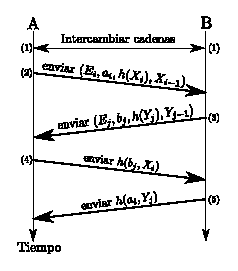
\includegraphics[scale=1.8]{imagenes/seguridad/exchange.eps}}{fig:fawkes}
{Elaboración propia, (2015)}


De esta manera, el protocolo asegura que ni $A$ ni $B$ puedan cambiar $E_i$
($E_j$) debido a que su contraparte se ha comprometido con una palabra código
que no ha sido aún publicada en texto plano. De igual manera, ninguno de los dos
pueden enviar otra palabra código diferente de $X_i$ ($Y_i$) debido a que su
\textit{hash} se encontraba en $a_i$ ($b_j$). Una tercera parte observando la
comunicación puede comprobar las fuentes y la integridad de los mensajes.

Ahora, si un nodo $A$ quiere saber que tan confiable es un nodo $B$ para enviar
el mensaje, debe validar la cadena de \textit{hashs} de $B$ utilizando aquellos
nodos de la cadena intercambiados previamente. Esto significa que algunos nodos
de la cadena puede que nunca sean validados si es que no se encuentra con la
entidad que los generó.

Lo expuesto anteriormente basta para probar si es que una interacción realmente
sucedió, con quien y evitar que se puedan generar unilateralmente
\textit{tickets} para mejorar las métricas del nodo. Para mitigar los ataques de
agujero negro, las interacciones consisten en \textit{tickets} de encuentro que
testifican las métricas internas del nodo, entregando información sobre la
calidad de conectividad que tiene el nodo, y en \textit{tickets} de transmisión
que indican la calidad del nodo para transmitir mensajes y evitan que un nodo
realice un ataque de agujero negro con \textit{tailgating}.

Para evitar un alto \overhead{} del protocolo adicional al intercambio de
mensajes de comunicación de los usuarios, en los encuentros posteriores
solamente se intercambian las diferencias entre los nodos de la cadena
de \textit{hash}.



\newpage
\subseccion{Protocolo de encaminamiento}
La información de los \textit{tickets} de interacción es validada por el
protocolo anterior, pero para la decisión de transmitir un mensaje de
comunicación a otro se basa en el conocimiento que se tiene del comportamiento
del nodo a ser examinado para ver su valor como portador del mensaje. El modelo
consiste en lo siguiente:

\begin{itemize}
  \item Interacciones antiguas tienen menos impacto que las nuevas. Esto permite
    descubrir si un nodo ha cambiado su comportamiento recientemente.
  \item Los \textit{tickets} de un mismo nodo que hayan ocurrido en una ventana
    de tiempo solo cuentan como uno. Esto permite evitar que nodos deshonestos
    generen una gran cantidad de \textit{tickets} mediante \textit{tailgating} y
    traten de hacerse pasar por un nodo honesto.
  \item Nodos con una alta movilidad en la red van a tender a tener una gran
    cantidad de \textit{tickets} de encuentros. Por ejemplo, en el contexto de
    un escenario de desastre como PDM, existen vehículos como ambulancias o
    patrullas de policía que recorren todo el escenario encontrándose con una
    alta cantidad de nodos. El protocolo, al momento de encaminar, debería tener
    esto en cuenta dado que es más probable que este tipo de nodos puedan llevar
    mensajes de comunicación a lugares distantes de la red.
  \item Nodos que colaboran con el proceso de transmisión de mensajes de
    comunicación van a tener una alta cantidad de \textit{tickets} de
    transmisión. Si un nodo no colabora con el enrutamiento de mensajes,
    entonces es probable que esté realizando un ataque de agujero negro o que
    sea un mal candidato a distribuir mensajes por la red.
\end{itemize}

El protocolo de enrutamiento en general está basado en \textit{Encounter-Based
Routing} (EBR) \cite{ebr}, especialmente en el cálculo de métricas una vez los
\textit{tickets} hay sido validados en su cadena de \textit{hashs}.


Se define una métrica llamada valor de encuentro o \textit{Encounter Value}
($EV_n$) para un nodo $n \in N$ en particular. Este valor se incrementa cada vez
que hay un nuevo \textit{ticket} de encuentro de un nodo validado. Se le da un
peso a cada \textit{ticket} para asignarle más valor a los encuentros más
recientes. El valor del peso ($w \in [0, 1]$) está relacionado con el
\textit{timestamp} de cada uno de los \textit{tickets} de encuentros. Por
ejemplo, un \textit{ticket} que es considerado antiguo tiene un valor de $w <
1$, y uno más reciente se le asignaría $w = 1$.


Se define adicionalmente una segunda métrica llamada valor de transmisión
o \textit{Transmission Value} ($TV_n$), que se computa de manera parecida a $EV$
pero esta vez para los \textit{tickets} de transmisión.


Para combinar ambas métrica se define la constante $\beta \in [0, 1]$ como un
peso de los parámetros $EV_n$ y $TV_n$ como se muestra a continuación:

\begin{equation}
  RV_n = EV_n * \beta + TV_n * (1 - \beta)
  \label{eq:valores_encuentro}
\end{equation}

Donde $RV_n$ es el valor de encaminamiento (\textit{Routing Value}) de un nodo
$n \in N$ en particular. Si se tiene un valor de $\beta$ alto, entonces se
consideran menos los \textit{tickets} de transmisión en la decisión de
encaminamiento, es decir, tienen menos influencia. En cambio, si $\beta$ es bajo, entonces
se le da más importancia a los \textit{tickets} de transmisión. El valor
adecuado de $\beta$ fue encontrado mediante pruebas en la sección de
experimentos.


Luego, de igual forma que EBR, se comparan las métricas de los $N$ nodos que
interactuaron con el nodo actual $c \in N$ (\textit{current node}). Al momento
de decidir si transmitir el mensaje o no, se compara el valor de encaminamiento
local ($c$) con el valor de encaminamiento del nodo a ser evaluado ($n$). Si el
nodo $n$ tiene un mayor $RV$ que el nodo $c$, entonces el mensaje es transmitido
debido a que tiene una mejor conectividad, en caso contrario el mensaje es
conservado. Esta decisión puede ser vista en la ecuación
(\ref{eq:fawkes_routing}) donde si el valor resultado es $> 1$ se transmite el
mensaje, $RV_c$ es el valor de encaminamiento del nodo $c$, $RV_n$ el valor de
encaminamiento del nodo $n$ y $r_i$ es la cantidad de réplicas restantes del
mensaje $i$ que puede hacer el nodo $n$, siendo esta una restricción similar a
la realizada por \syw{} para limitar la cantidad de copias en la red.



\begin{equation}
  \left\lfloor \frac{RV_n*r_i}{RV_c+RV_n} \right\rfloor > 1
  \label{eq:fawkes_routing}
\end{equation}


\seccion{Evaluación de \textit{FawkesRouter}}


El protocolo de seguridad fue evaluado respecto a métricas como la tasa de
entrega, \overhead{} y latencia de mensajes, energía consumida en las
transmisiones y número de mensajes que logran ser atraídos a un agujero negro
con diferentes niveles de nodos maliciosos. Se compara el desempeño de los nodos
con protocolos de encaminamiento como \syw{} \cite{spyropoulos_spray_2005},
\syf{} \cite{spyropoulos_spray_2007}, \prophet{} y \maxprop.

\subseccion{Parámetros de simulación}
Se utiliza el simulador \theone{} \cite{keranen_one_2009} para la evaluación del
protocolo sobre dos modelos de movilidad: \textit{Working Day Movement Model}
(WDMM) \cite{ekman_working_2008} y \textit{Post Disaster Mobility Model}. Se
utilizaron estos dos debido a que capturan los diferentes movimientos que
existen en una ciudad, el primero en el día a día y el segundo luego de un
desastre.

El primer escenario utiliza WDMM y simula $345600$ segundos (4 días)
considerando un día de trabajo de $8$ horas. La red se compone de 150 nodos que
se mueven por la ciudad de \textit{Helsinki}, Finlandia. Los otros parámetros
utilizados son los propuestos por el modelo de movilidad en
\cite{ekman_working_2008}.  Cada mensaje tiene un tamaño de $25$ KB y un mensaje
es generado cada minuto de la simulación.

El segundo escenario utiliza PDM con las configuraciones propuestas en
\cite{uddin_post-disaster_2009}. Se ha simulado un escenario de desastre de $172000$
segundos o $47$ horas compuesto por $10$ vecindarios con $20$ personas cada
uno, un centro de comando, $5$ centros de suministros, $1$ centro médico con $5$
ambulancias, $1$ centro de policía con $5$ patrullas, $1$ vehículo de reparación
de carreteras, $20$ rescatistas y $60$ casas. Cada uno de estos tipos de nodos
se mueve de acuerdo a las reglas establecidas por $PDM$. Los mensajes en este
segundo escenario se generan cada $120$ segundos y tienen un tamaño de $500$ KB.

Ambos escenarios utilizan un TTL de $360$ minutos o $6$ horas y un tamaño de
buffer de $50$ MB.

Para simular ataques de agujero negros, se ha implementado un sistema dentro de los
nodos maliciosos para que ellos puedan descartar los mensajes pero permitiendo
que se muevan como cualquier otra persona participante honesta de la red.
Una vez que un nodo malicioso recibe un mensaje, simplemente lo descarta sin
siquiera guardarlo en el buffer, pero desde el punto de vista del nodo que envía
el mensaje la transferencia fue exitosa. Para evaluar el éxito de los nodos
maliciosos se cuentan la cantidad de mensajes que han sido capturados por el
atacante.


\subseccion{Resultados de las simulaciones}
Los primeros experimentos realizados están enfocados en descubrir cual es un valor de $\beta
\in [0, 1]$ adecuado para escoger en un protocolo, donde un valor cercano a $0$
significa que se le da más importancia a los \textit{tickets} de transmisión
mientras que un valor cercano a $1$ da más importancia a los \textit{tickets} de
transmisión. La intuición indica que $\beta$ debería tener un valor entre $0$ a
$0.5$, dado que en este contexto de ataque los \textit{tickets} de encuentros
son menos relevantes que los de transmisión, estos últimos utilizados para
averiguar si un nodo está o no realizando un ataque a la red. 

Se mide el éxito del protocolo creado de acuerdo a la cantidad de mensajes que
se logran evitar que caigan en un nodo malicioso, siendo un ataque satisfactorio
si se atraen a un nodo malicioso una alta cantidad de mensajes o si todas las
copias de un mensaje se pierden perjudicando la tasa de entrega. A pesar que se
presentan en las pruebas porcentaje de nodos maliciosos de 0\% a 90\%, tener una
cantidad de atacantes igual o mayor a 50\% no es realista debido a que en ese
caso más de la mitad de la red se encuentra realizando el ataque lo que
significa que la cantidad de nodos viables que pueden ser utilizados para enviar
los mensajes son menos del 50\%.

En la definición de la fórmula que relaciona el valor de encuentro de los
\textit{tickets} de transmisión y los de comunicación en la Ecuación
\ref{eq:fawkes_routing}, se puede ver que con un valor de $\beta = 1$ el
protocolo se comporta igual que EBR.

En la \ref{fig:delivery-busqueda-beta-wdmm},
\ref{fig:latencia-busqueda-beta-wdmm} y \ref{fig:atraidos-busqueda-beta-wdmm} se
pueden ver los resultados de las simulaciones de \textit{FawkesRouter} para
distintos valores de $\beta$ en el modelo de movilidad WDMM. Para un valor de
$\beta = 0$ es cuando se obtiene el peor desempeño debido a que solamente se
están considerando los \tickets{} de transmisión para tomar la decisión de pasar
o no el mensaje. A pesar que esto podría parecer lo mejor para evitar ataques de
agujero negro, el problema que surge es que nunca se envían los mensajes debido
a que nunca se generan \textit{tickets} de transmisión debido a que al inicio de
la simulación, aún no se envía ningún mensaje, lo que hace que se comporte igual
para todos los valores de \% de nodos maliciosos. El pequeño valor de la tasa de
entrega para este caso es causado por entregas uno a uno, es decir, entregas de
mensajes cuando el nodo se encuentra directamente con el destino.

Para otros valores de $\beta$, se puede ver que el desempeño es similar entre
ellos. Todos comienzan a bajar su desempeño a medida que aumenta la cantidad de
nodos maliciosos, pero hay unos que tienen mayor tasa de entrega. En el caso de
$\beta = 1$, se obtiene la mejor tasa de entrega, pero al un alto costo como se
puede ver en la \ref{fig:atraidos-busqueda-beta-wdmm} donde es el protocolo con
mayor cantidad de mensajes atraídos por los atacantes, lo que implica mayor
consumo de energía al transmitir los mensajes.

Por el lado de la latencia, presentado en la
\ref{fig:latencia-busqueda-beta-wdmm}, hay una diferencia en promedio de 20
segundos entre el mejor y el peor protocolo. El mejor tiempo obtenido por
protocolos cercanos a $\beta = 1$ se debe a que ellos tienden a enviar los
mensajes sin importar los \tickets{} de transmisión, es decir, sin tomar en
cuenta si un nodo es un potencial atacante o no, por lo que son menos precavidos
que otros nodos y aprovechan más oportunidades de entregar los mensajes.

La forma de las curvas de la \ref{fig:atraidos-busqueda-beta-wdmm} se debe
principalmente a que los nodos maliciosos se perjudican entre ellos y a medida
que más de la mitad de la red participa en el ataque, entonces también hay menos
mensajes disponibles para ser atraídos, es por esto que a partir del 50\%, hay
menos mensajes atraídos, porque hay menos mensajes que tienen la posibilidad de
ser copiados al ser atraídos inmediatamente a un agujero negro.


\figuraFuente{Tasa de entrega en WDMM para distintos $\beta$.}
{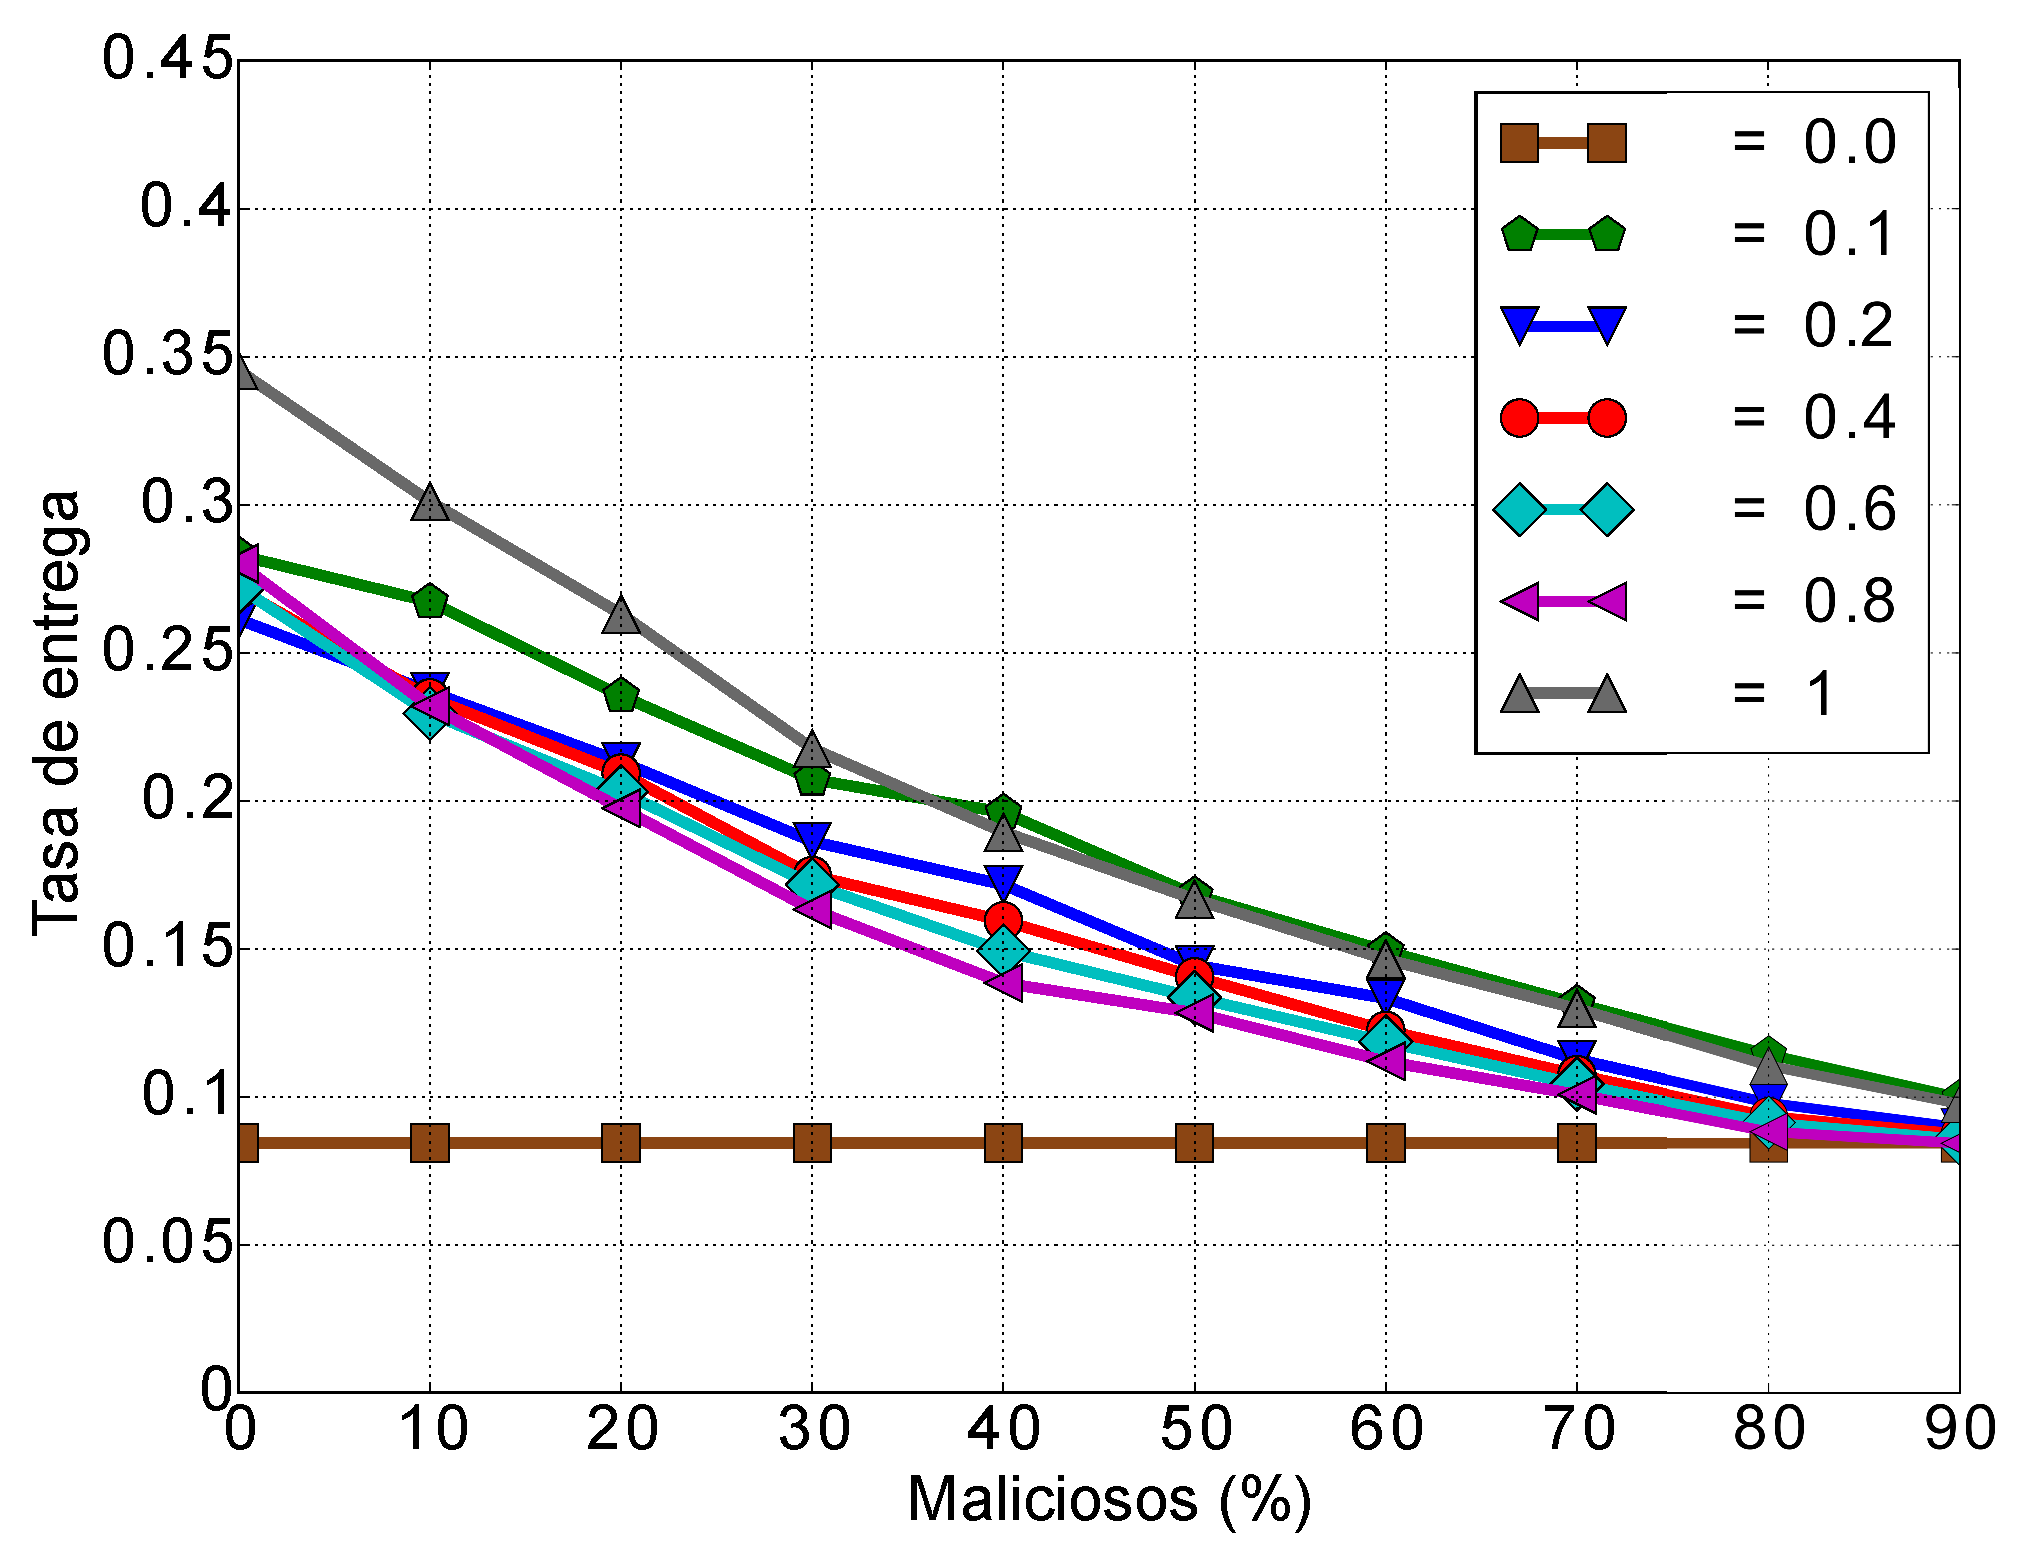
\includegraphics[width=0.6\textwidth]{imagenes/seguridad/graficos/delivery_busqueda_beta.eps}}{fig:delivery-busqueda-beta-wdmm}
{Elaboración propia, (2015)}

\figuraFuente{Latencia de los mensajes en WDMM para distintos $\beta$.}
{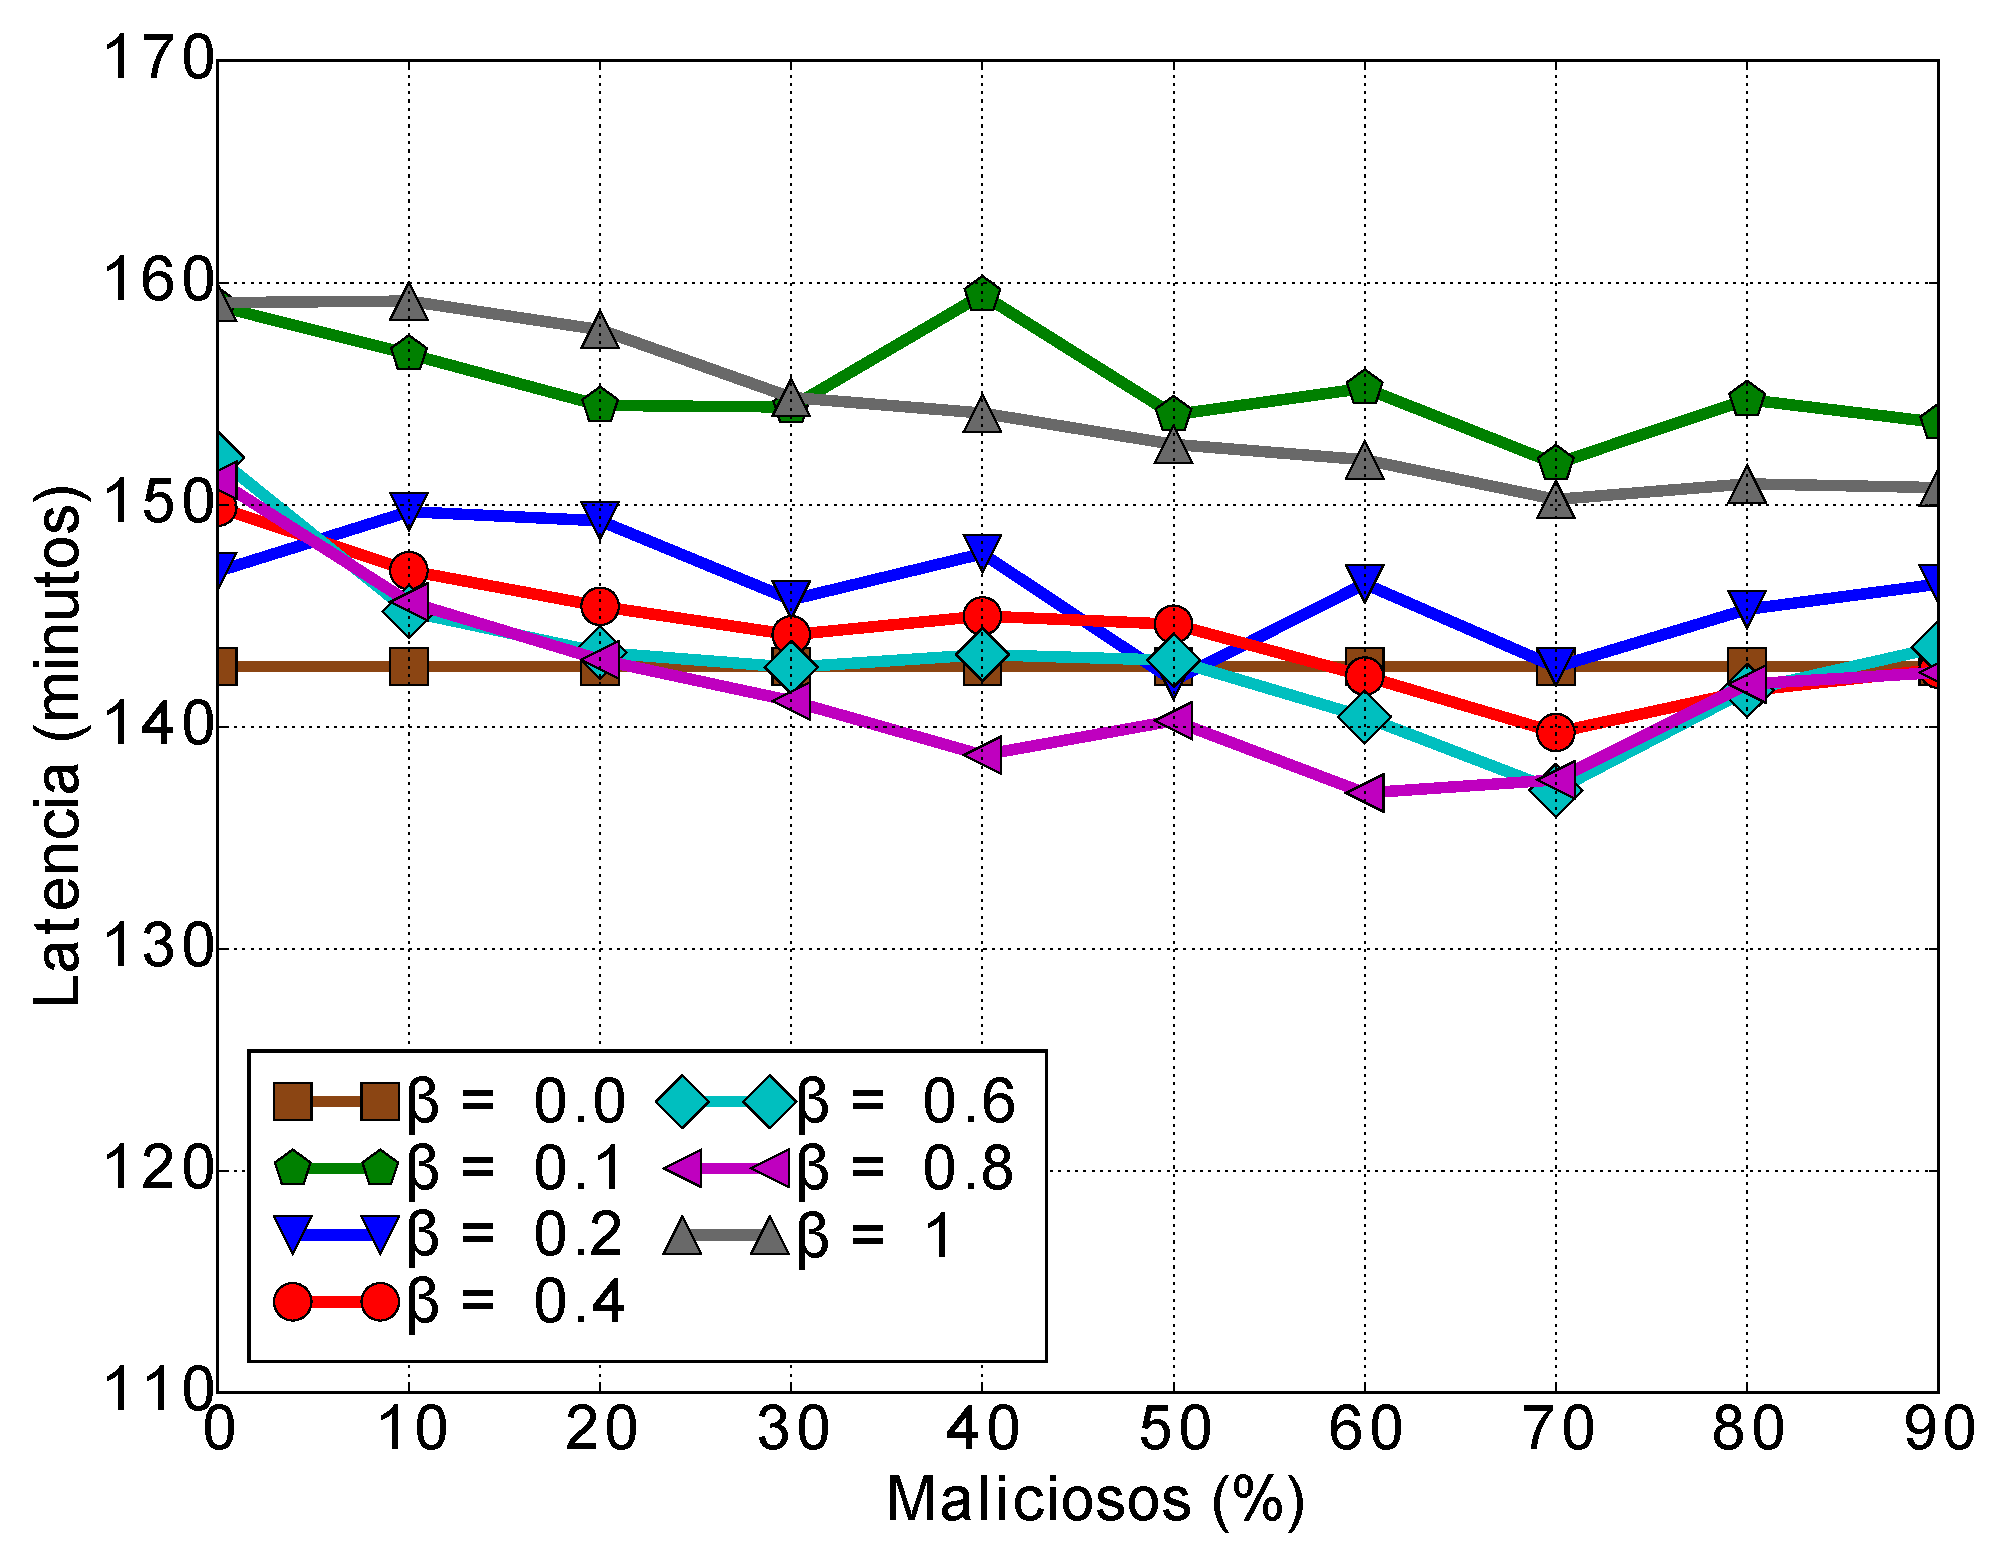
\includegraphics[width=0.6\textwidth]{imagenes/seguridad/graficos/latencia_busqueda.eps}}{fig:latencia-busqueda-beta-wdmm}
{Elaboración propia, (2015)}

\figuraFuente{Cantidad de mensajes atraídos a un agujero negro en WDMM para distintos $\beta$.}
{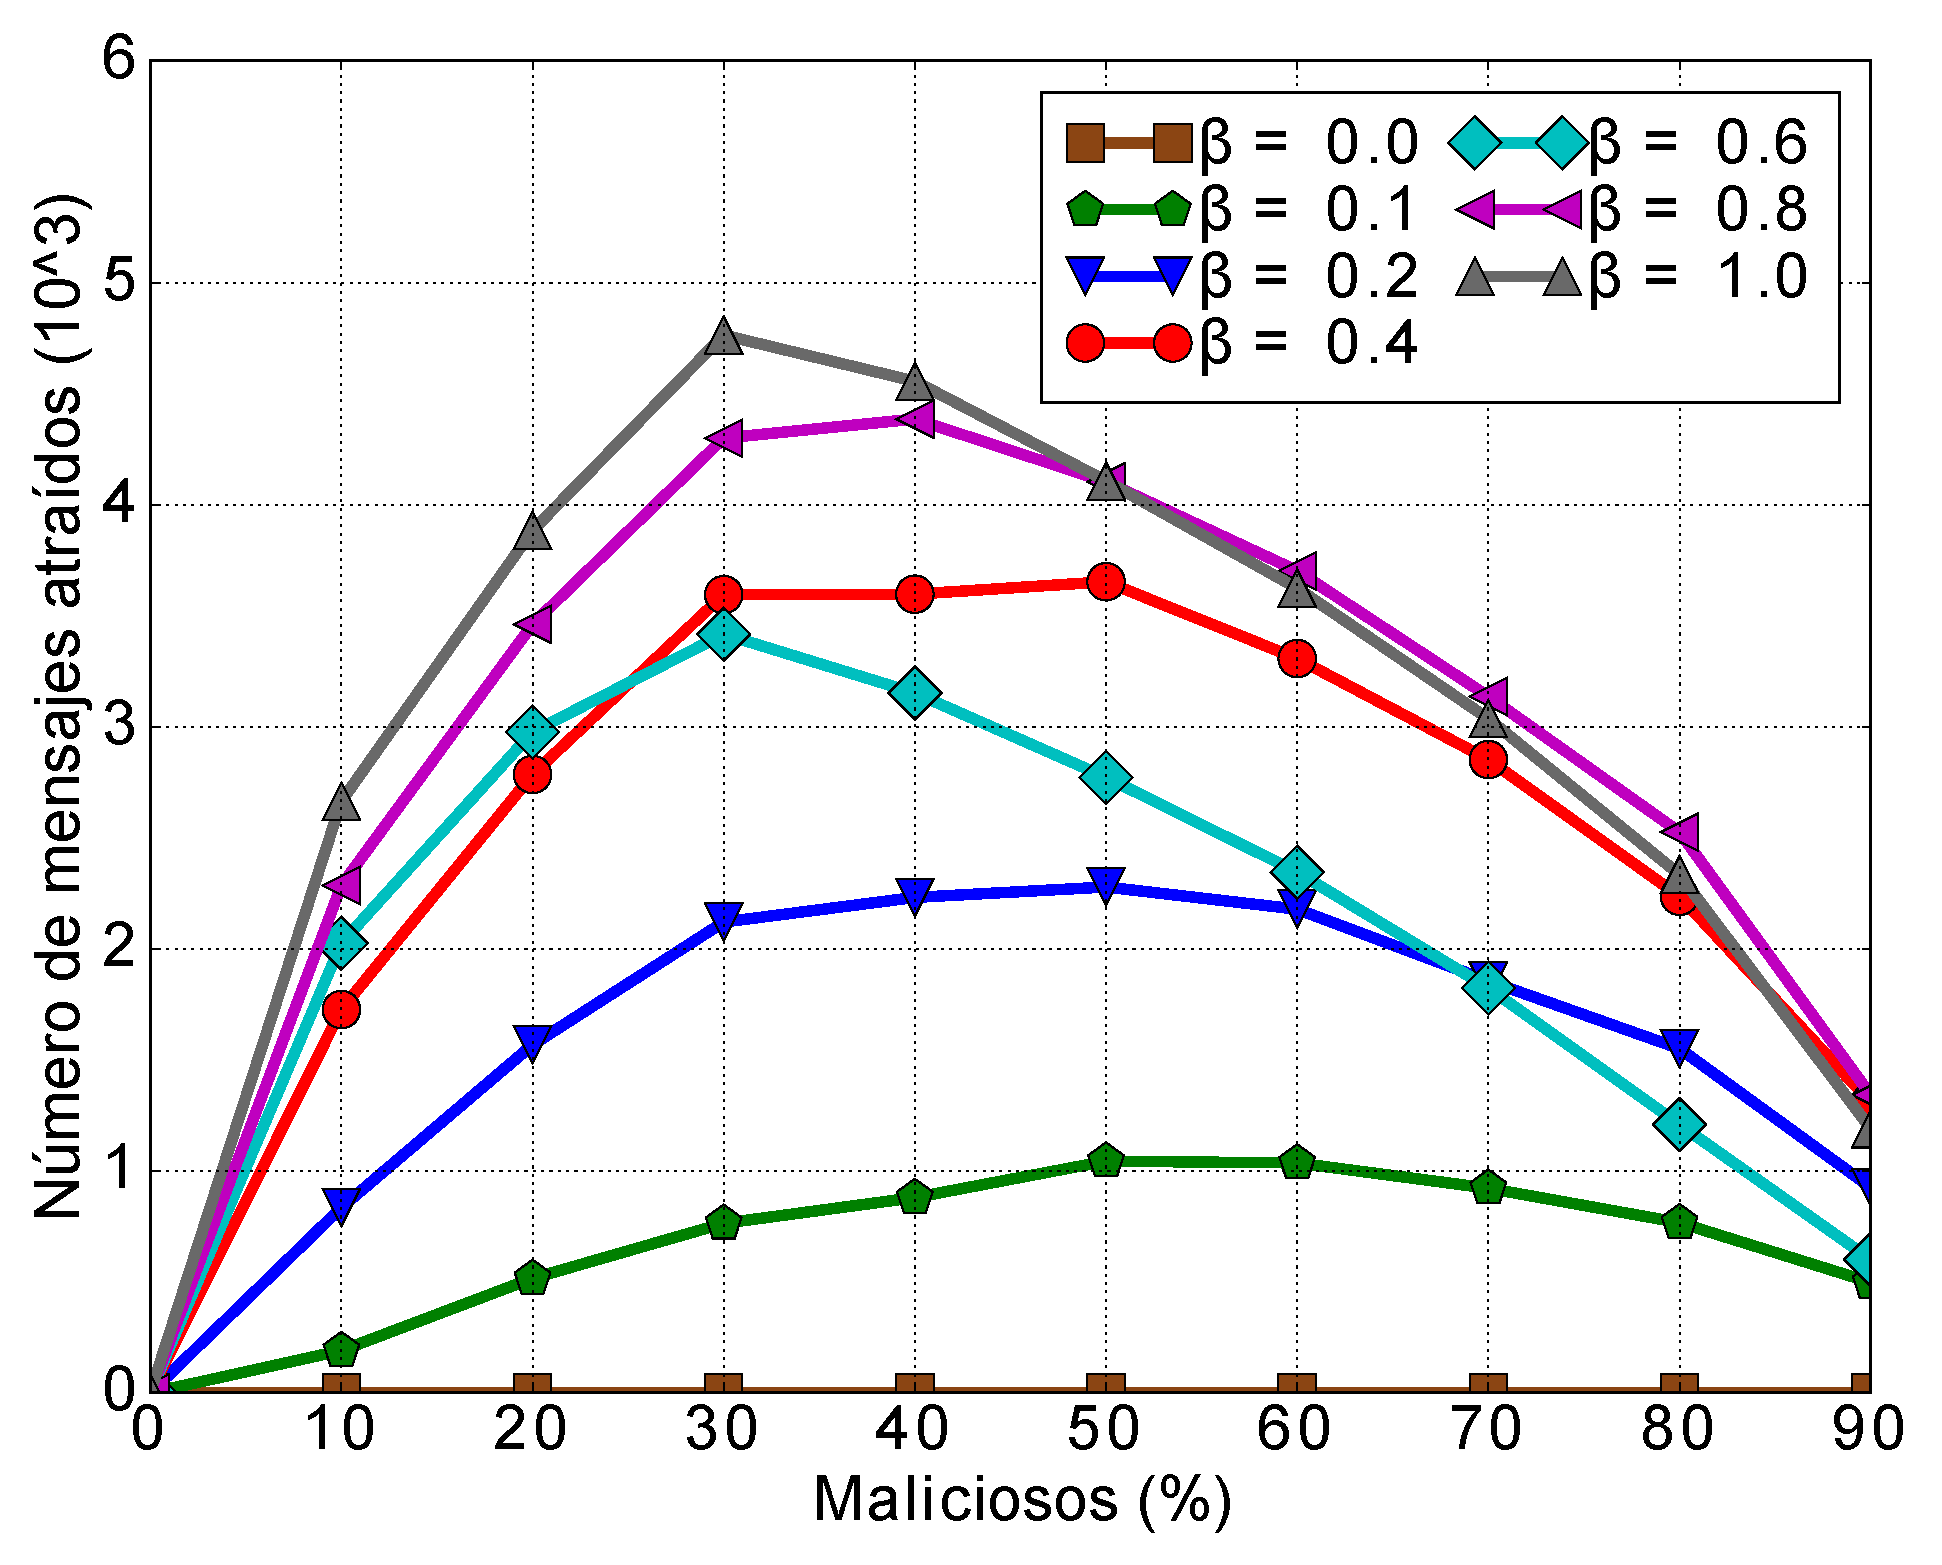
\includegraphics[width=0.6\textwidth]{imagenes/seguridad/graficos/atraidos_busqueda_beta.eps}}{fig:atraidos-busqueda-beta-wdmm}
{Elaboración propia, (2015)}

%%%%%%%%%%%%%%%%%%%%%%%%%%%%%%%%%%%%%%%%%%%%%%%%%%%%%%%%%%%%%%%%%%%%%%%%%%%%%%%%


En el caso de PDM, los resultados son similares. Nuevamente $\beta = 0$ tiene el
peor desempeño por la misma razón de antes que no envía nada porque no es capaz
de generar información para luego poder utilizarla para evaluarla. $\beta =
0.1$ supera en esta ocasión a $\beta = 1$ desde el 10 \% de nodo maliciosos. A
partir del 40\% en adelante, todos los protocolos se estabilizan y no siguen
bajando su tasa de entrega, lo cual es causado por la forma en la cual se están
asignando los nodos maliciosos en la simulación. Los nodos maliciosos en el caso
de este escenario están asignados solo a las personas quienes componen los
vecindarios debido a que es el punto más fácil de entrada para un atacante. Una
patrulla o ambulancia que realice un ataque significaría mayor dificultad debido
a que son nodos controlados por las autoridades. A medida que se aumenta la
cantidad de nodos maliciosos en los vecindarios, estos comienzan a aislarse
mutuamente, al igual que en WDMM, lo que reduce tanto la posibilidad de entregar
un mensaje (tasa de entrega) como la cantidad de mensajes que los atacantes
logran recolectar.



%%%%%%%%%%%%%%%%%%%%%%%%%%%%%%%%%%%%%%%%%%%%%%%%%%%%%%%%%%%%%%%%%%%%%%%%%%%%%%%%

\figuraFuente{Tasa de entrega en PDM para distintos $\beta$.}
{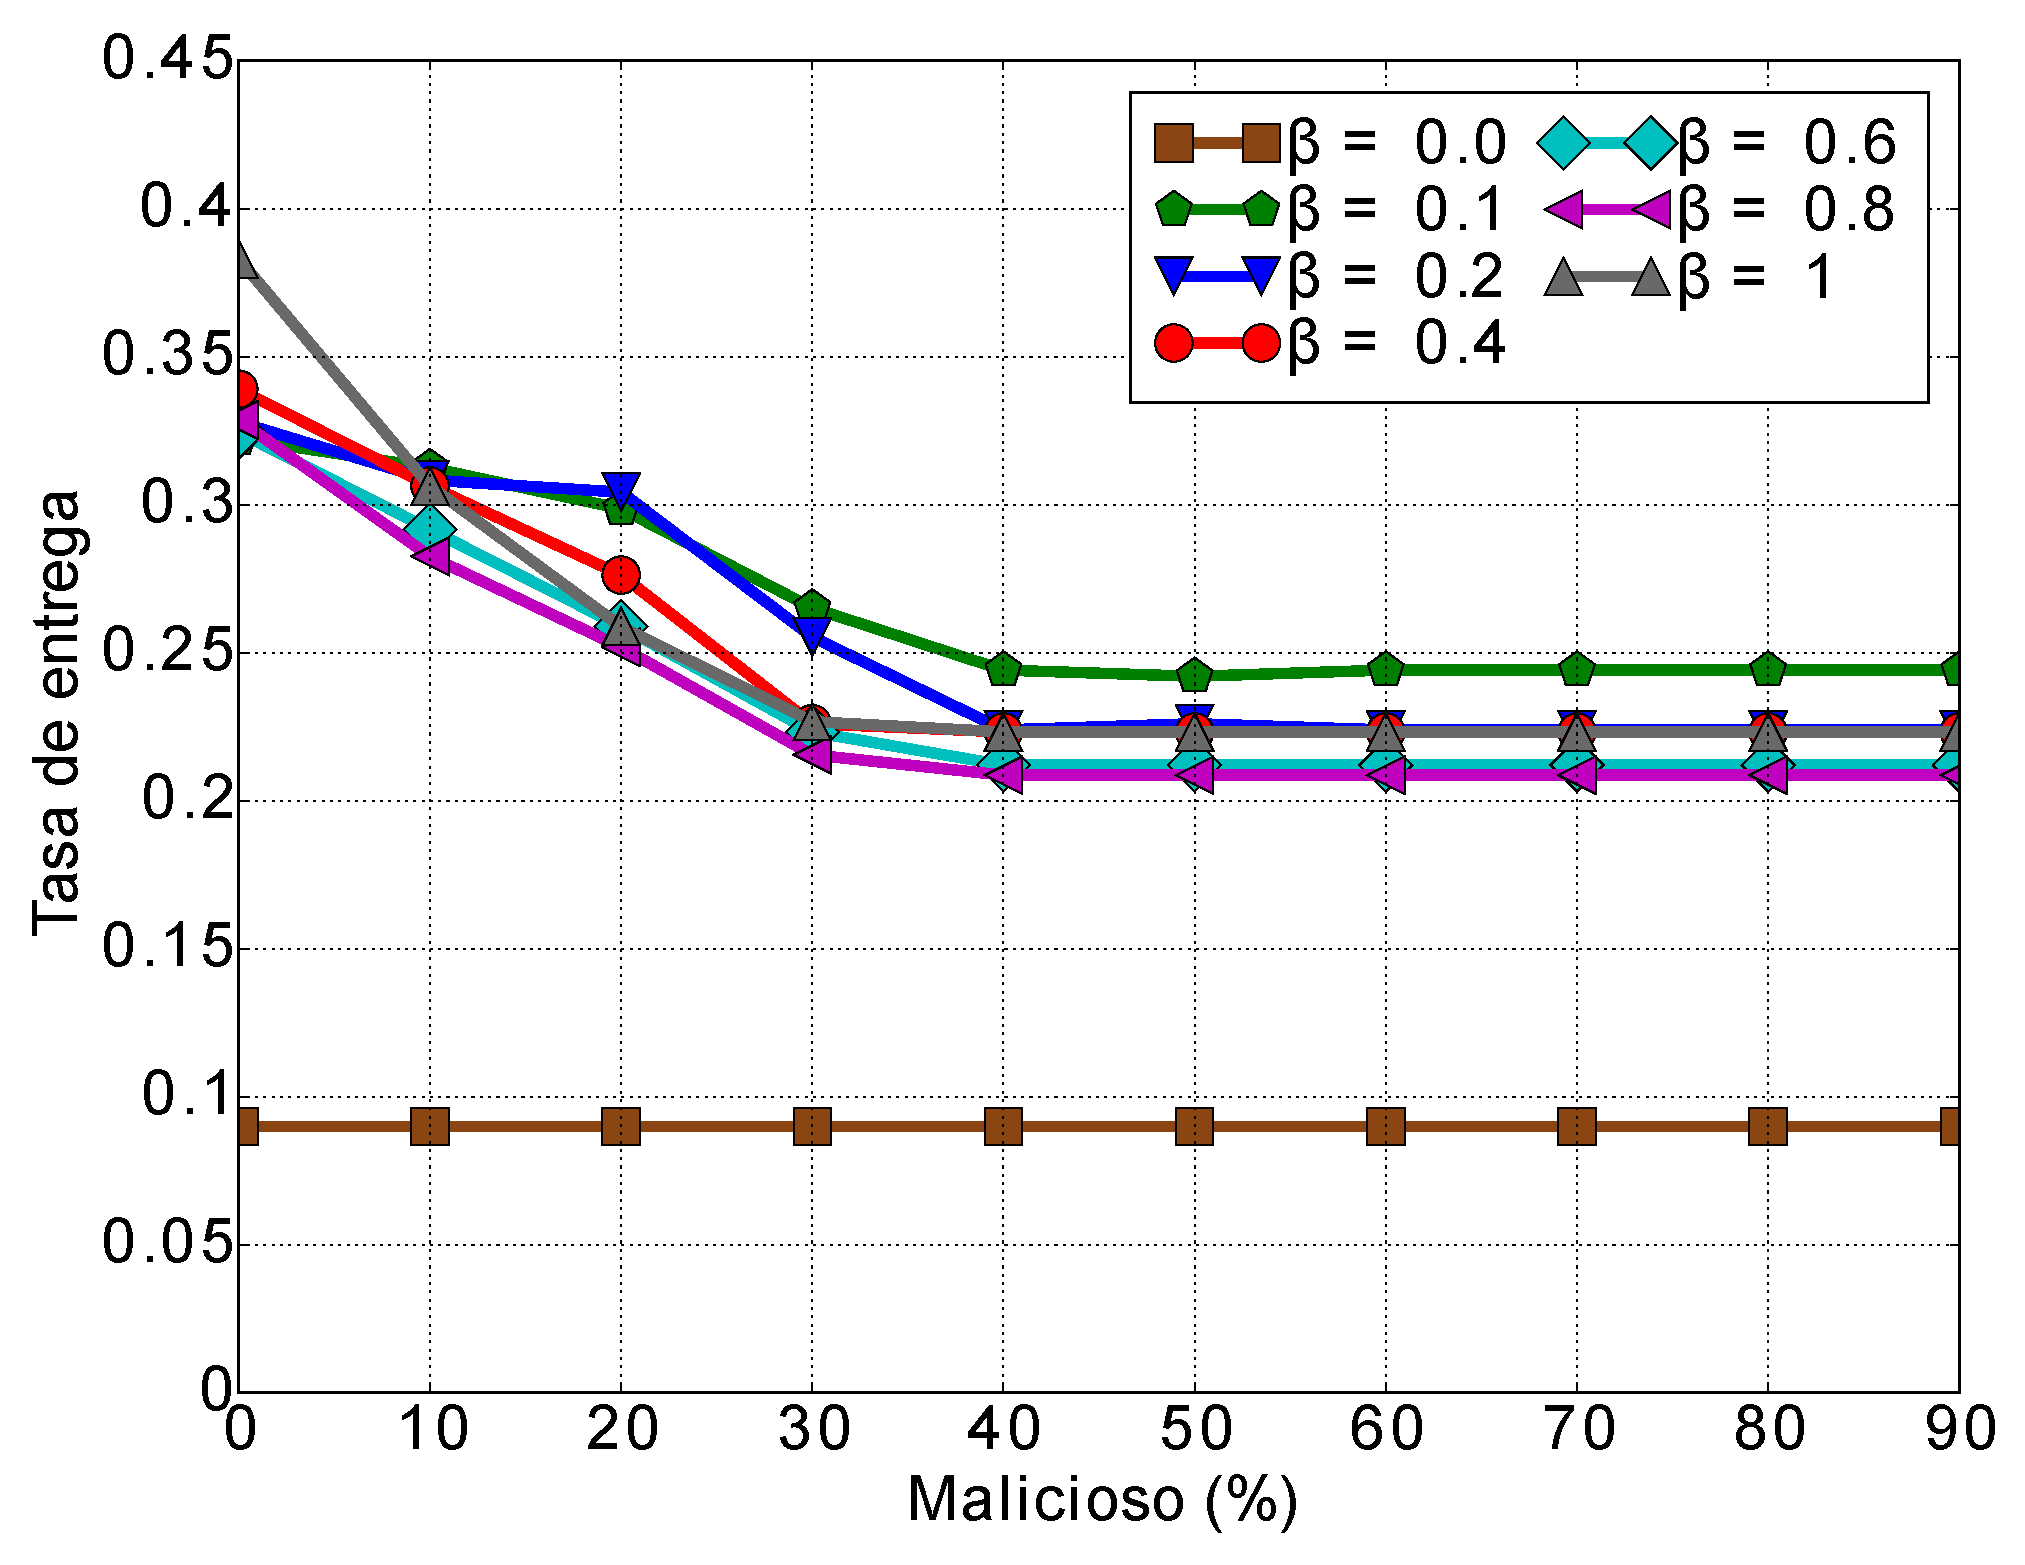
\includegraphics[width=0.6\textwidth]{imagenes/seguridad/graficos/delivery_pdm_ebr.eps}}{fig:delivery-busqueda-beta-pdm}
{Elaboración propia, (2015)}

\figuraFuente{Latencia de los mensajes en PDM para distintos $\beta$.}
{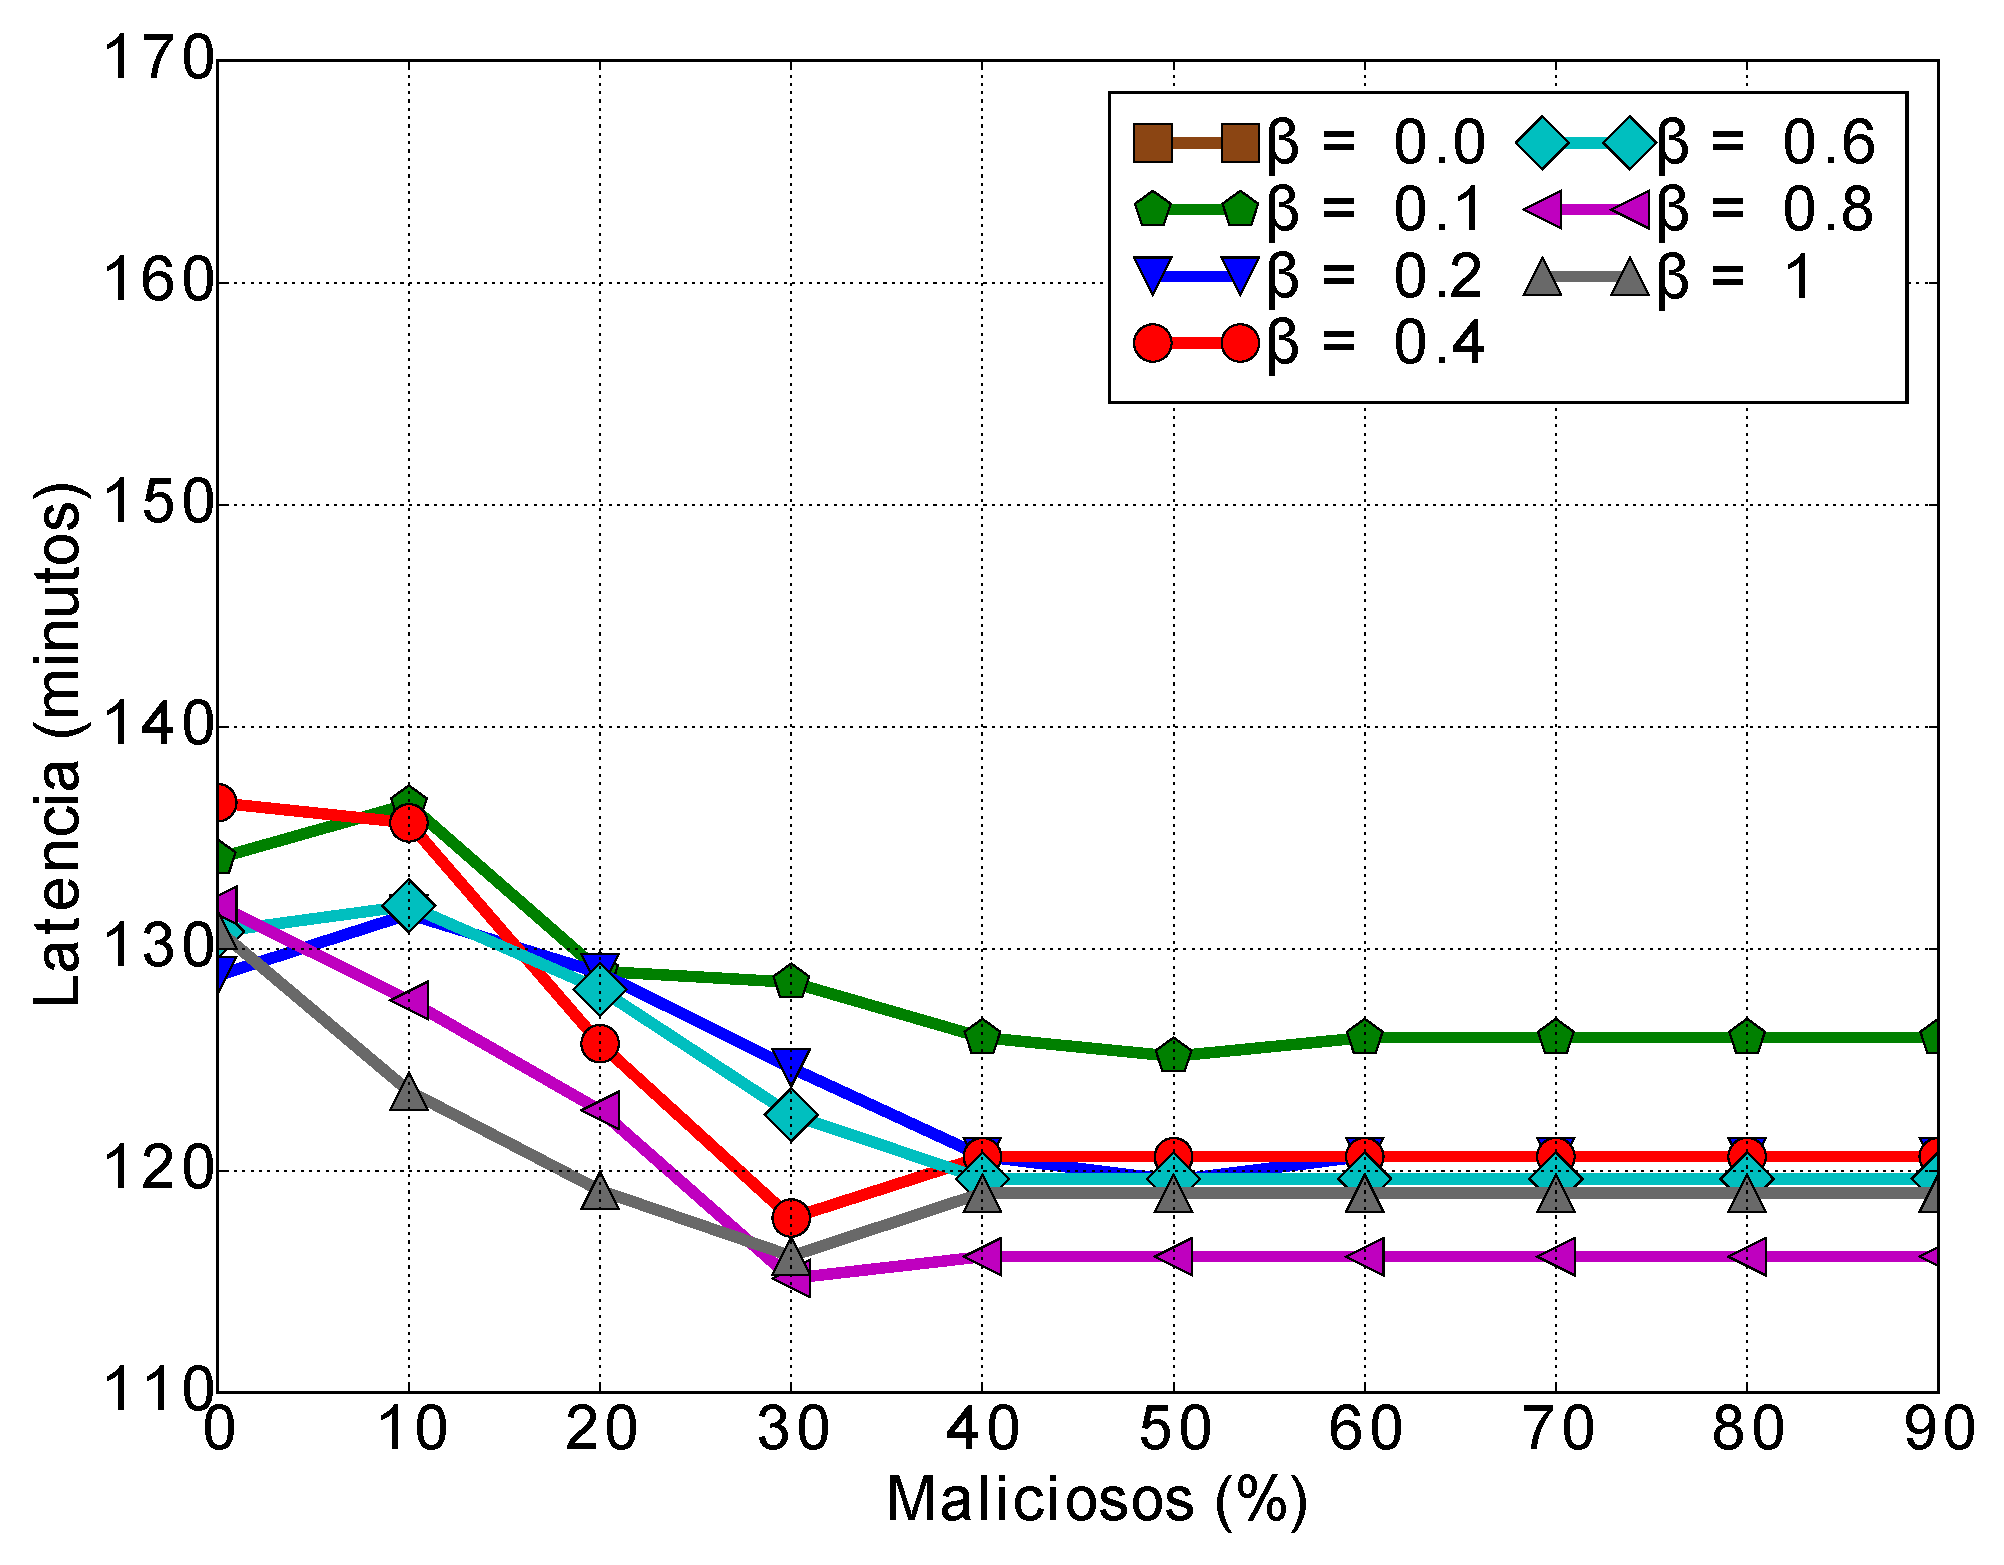
\includegraphics[width=0.6\textwidth]{imagenes/seguridad/graficos/latency_pdm_ebr.eps}}{fig:latencia-busqueda-beta-pdm}
{Elaboración propia, (2015)}

\figuraFuente{Cantidad de mensajes atraídos a un agujero negro en PDM para distintos $\beta$.}
{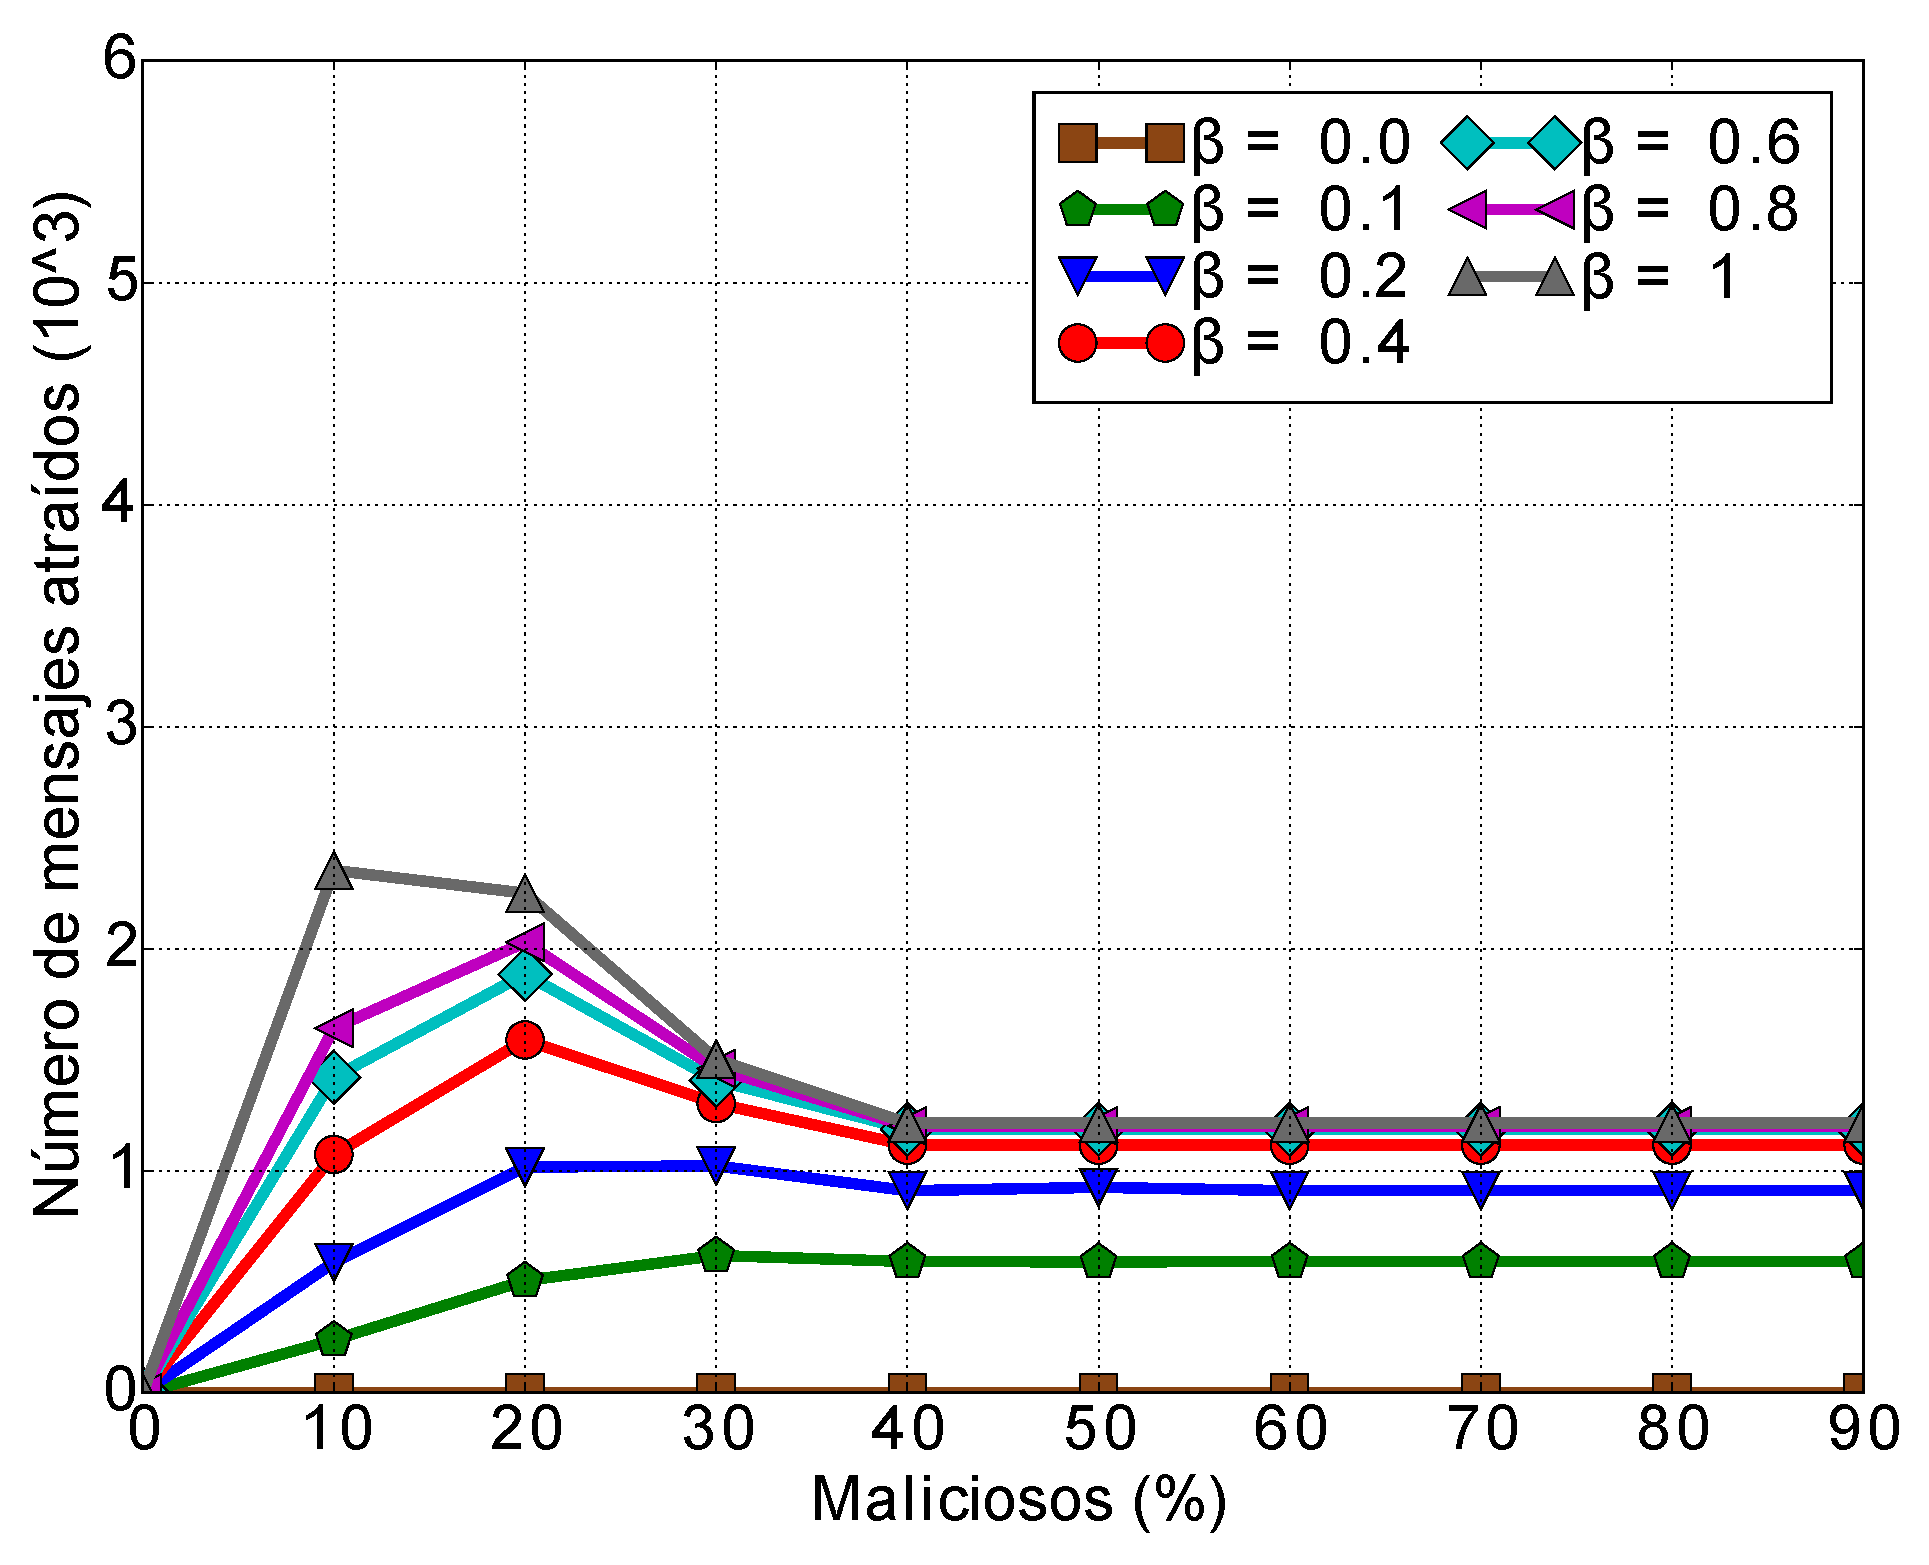
\includegraphics[width=0.6\textwidth]{imagenes/seguridad/graficos/atraidos_pdm_ebr.eps}}{fig:atraidos-busqueda-beta-pdm}
{Elaboración propia, (2015)}


%%%%%%%%%%%%%%%%%%%%%%%%%%%%%%%%%%%%%%%%%%%%%%%%%%%%%%%%%%%%%%%%%%%%%%%%%%%%%%%%

Una vez realizados estos experimentos se puede analizar más detalladamente el
valor que debería tener $\beta$. Entre ambos modelos de movilidad los valores
que más destacan son $\beta = 1$, $\beta = 0.1$ y $\beta = 0.2$. El primer caso
solamente toma en cuenta los \tickets{} de encuentro dejando de lado los de
transmisión lo que causa que un alto número de mensajes sean atraídos por los
agujeros negros creando un alto consumo de energía de comunicación. 

Finalmente se decide escoger $\beta = 0.2$ debido a que es el protocolo que
presenta la mejor concesión entre tasa de entrega, latencia y cantidad de
mensajes atraídos, donde el valor de $0.2$ es comparable con el de $0.1$,
teniendo una mayor cantidad de mensajes atraídos por nodos maliciosos pero una
mejor latencia.

A continuación se presentan los resultados obtenidos al utilizar
\textit{FawkesRouter} con $\beta = 0.2$ comparándolo con protocolos del estado
del arte, específicamente \epidemic, \prophet, \syw, \syf{} y \maxprop.


En las \ref{fig:delivery-protocolos-wdmm}, \ref{fig:overhead-protocolos-wdmm} y
\ref{fig:atraidos-protocolos-wdmm} se pueden ver los resultados al comparar los
protocolos para el modelo de movilidad WDMM, cambiando en este caso la métrica
de latencia por la de \overhead{} que se relaciona directamente con el consumo
de energía como se mostró en la ecuación (\ref{eq:energia}). \syf{}
presenta la mejor tasa de entrega entre 0\% y 70\%, menor \overhead{} de
mensajes pero al costo de tener la mayor cantidad de mensajes atraídos por los
nodos maliciosos. Esto quiere decir que en WDMM, \syf{} es el protocolo más
afectado por el ataque de agujero negro. Por otro lado, \textit{FawkesRouter}
tiene un delivery ratio similar a \syw{} en este escenario junto con resultados
parecidos en \overhead{} y en cantidad de mensajes atraídos. Con estos
resultados no es posible identificar si es que \textit{FawkesRouter} es mejor o
peor que otros protocolos como \syw.




%%%%%%%%%%%%%%%%%%%%%%%%%%%%%%%%%%%%%%%%%%%%%%%%%%%%%%%%%%%%%%%%%%%%%%%%%%%%%%%%


\figuraFuente{Tasa de entrega en WDMM para distintos protocolos.}
{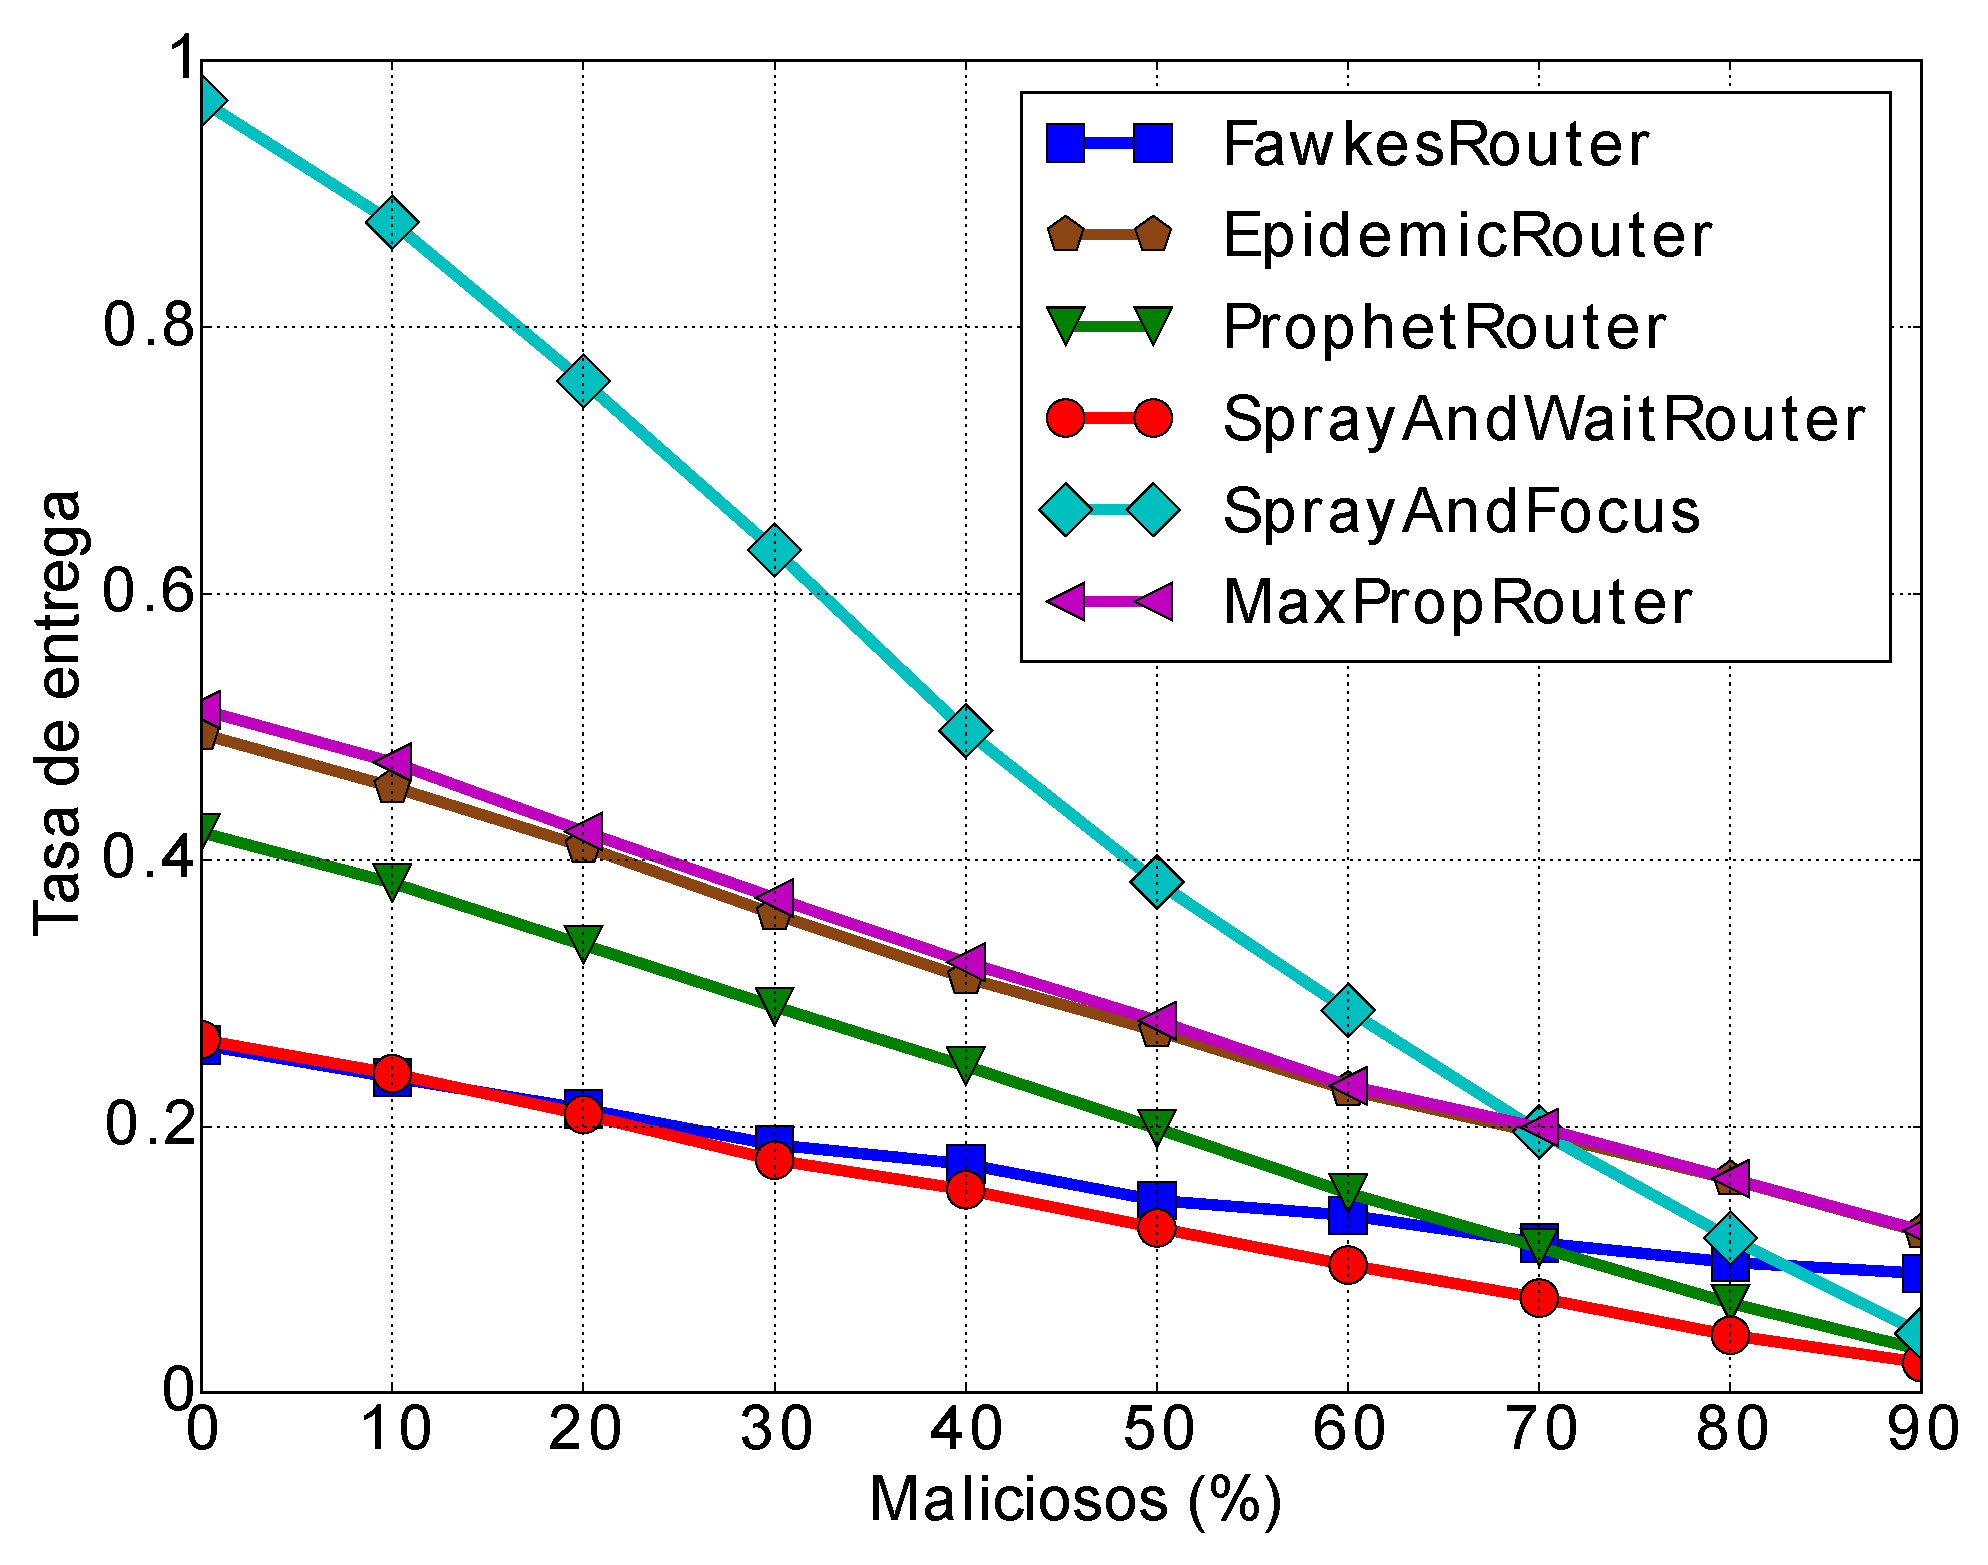
\includegraphics[width=0.6\textwidth]{imagenes/seguridad/graficos/delivery_comparacion.eps}}{fig:delivery-protocolos-wdmm}
{Elaboración propia, (2015)}

\figuraFuente{\textit{Overhead} en WDMM para distintos protocolos.}
{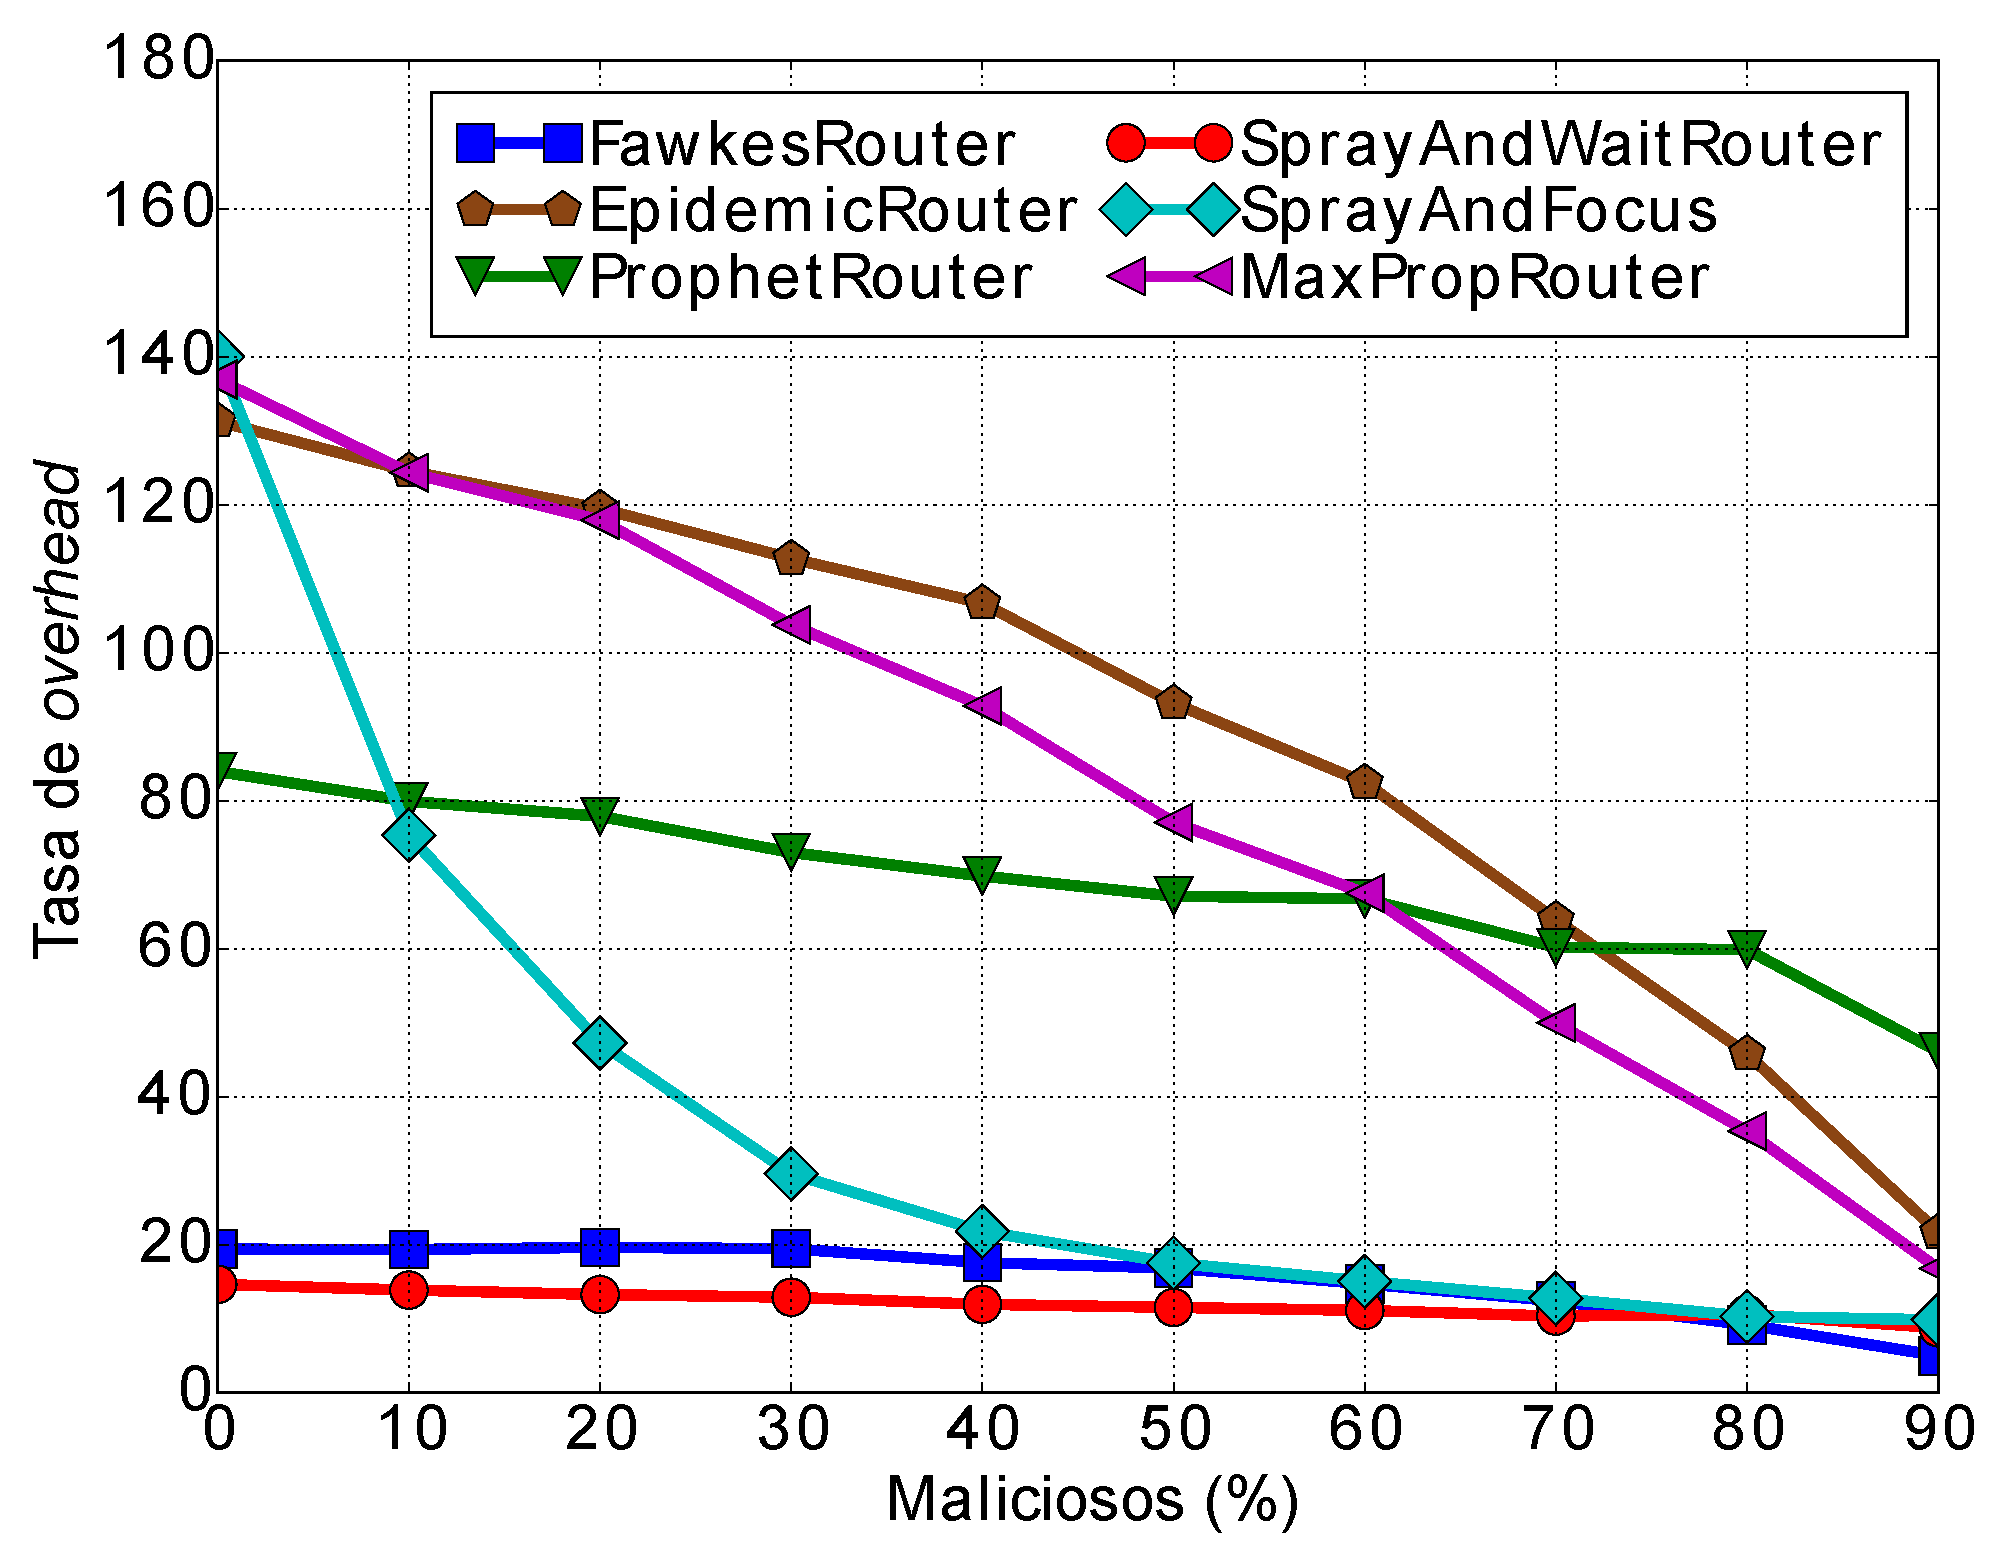
\includegraphics[width=0.6\textwidth]{imagenes/seguridad/graficos/overhead_comparacion.eps}}{fig:overhead-protocolos-wdmm}
{Elaboración propia, (2015)}

\figuraFuente{Cantidad de mensajes atraídos en WDMM para distintos protocolos.}
{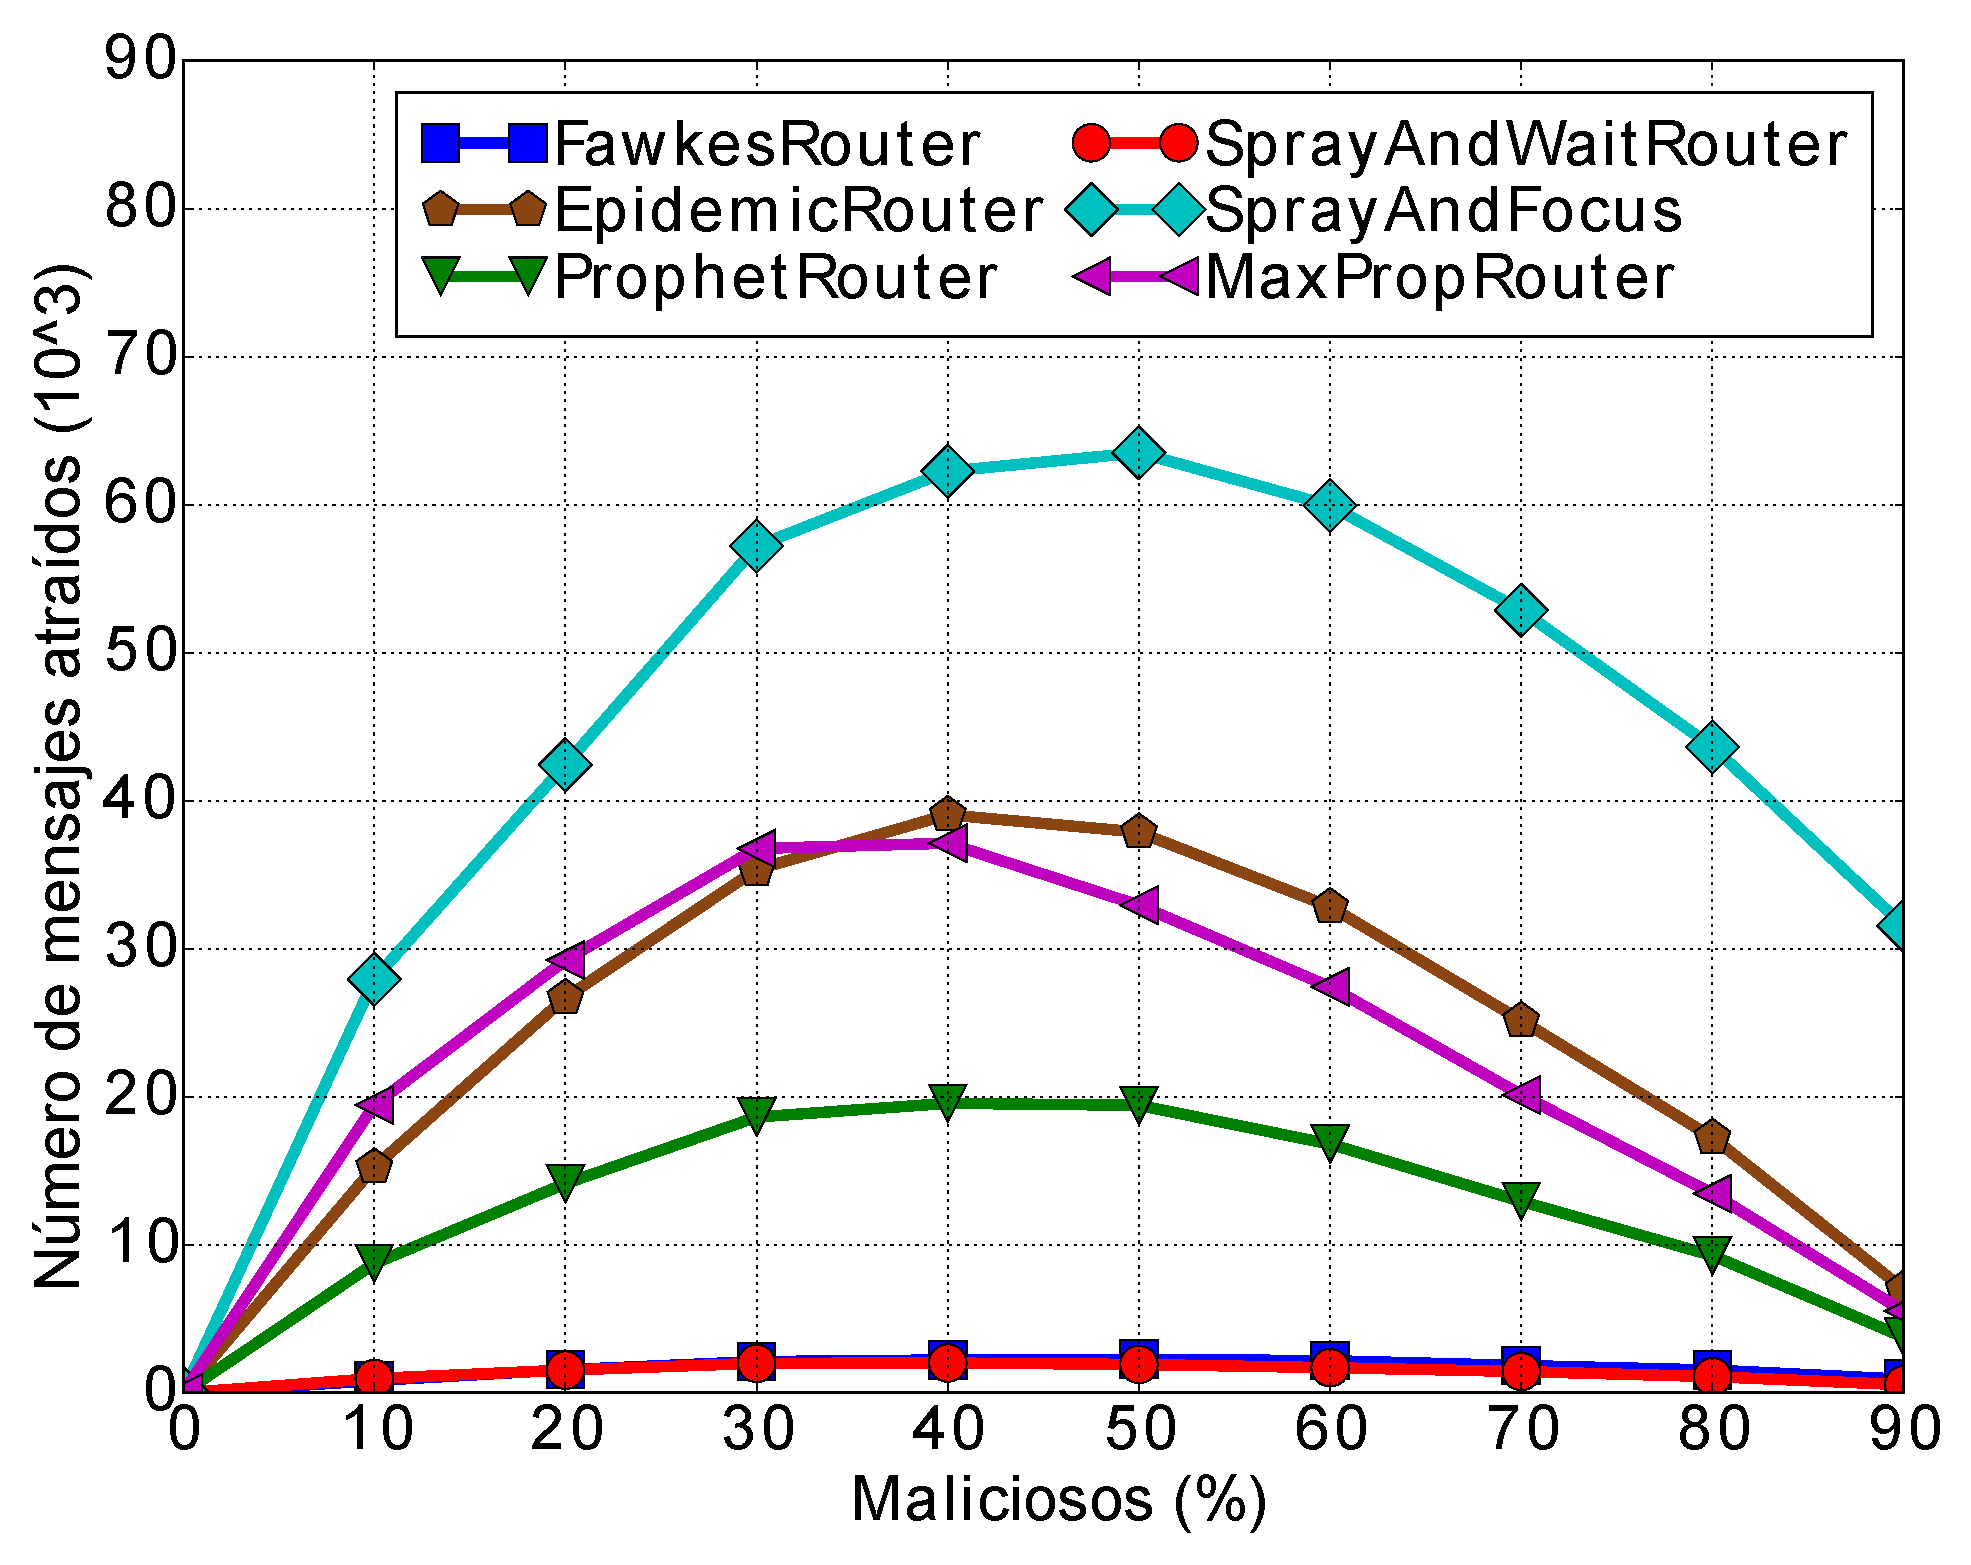
\includegraphics[width=0.6\textwidth]{imagenes/seguridad/graficos/atraidos_comparacion.eps}}{fig:atraidos-protocolos-wdmm}
{Elaboración propia, (2015)}


%%%%%%%%%%%%%%%%%%%%%%%%%%%%%%%%%%%%%%%%%%%%%%%%%%%%%%%%%%%%%%%%%%%%%%%%%%%%%%%%


En el escenario de PDM, mostrado en la \ref{fig:delivery-protocolos-pdm},
\ref{fig:overhead-protocolos-pdm} y \ref{fig:atraidos-protocolos-pdm},
presenta el desempeño de los protocolos en un escenario de post desastre. Se
puede ver que en esta ocasión \textit{FawkesRouter} tiene una mejor tasa de
entrega que \syf{} y \syw{}, manteniendo constante su desempeño a partir del
40\%. Otros protocolos, \prophet, \maxprop{} y \epidemic, tienen mejor tasa de
entrega que \textit{FawkesRouter}, pero incurren en un mayor \overhead{}
(\ref{fig:overhead-protocolos-pdm}) y por lo tanto en un mayor consumo de energía
de transmisión de mensajes. Este alto \overhead{} es causado por la alta
cantidad de mensajes que es atraído por los respectivos protocolos
(\ref{fig:atraidos-protocolos-pdm}).



%%%%%%%%%%%%%%%%%%%%%%%%%%%%%%%%%%%%%%%%%%%%%%%%%%%%%%%%%%%%%%%%%%%%%%%%%%%%%%%%


\figuraFuente{Tasa de entrega en PDM para distintos protocolos.}
{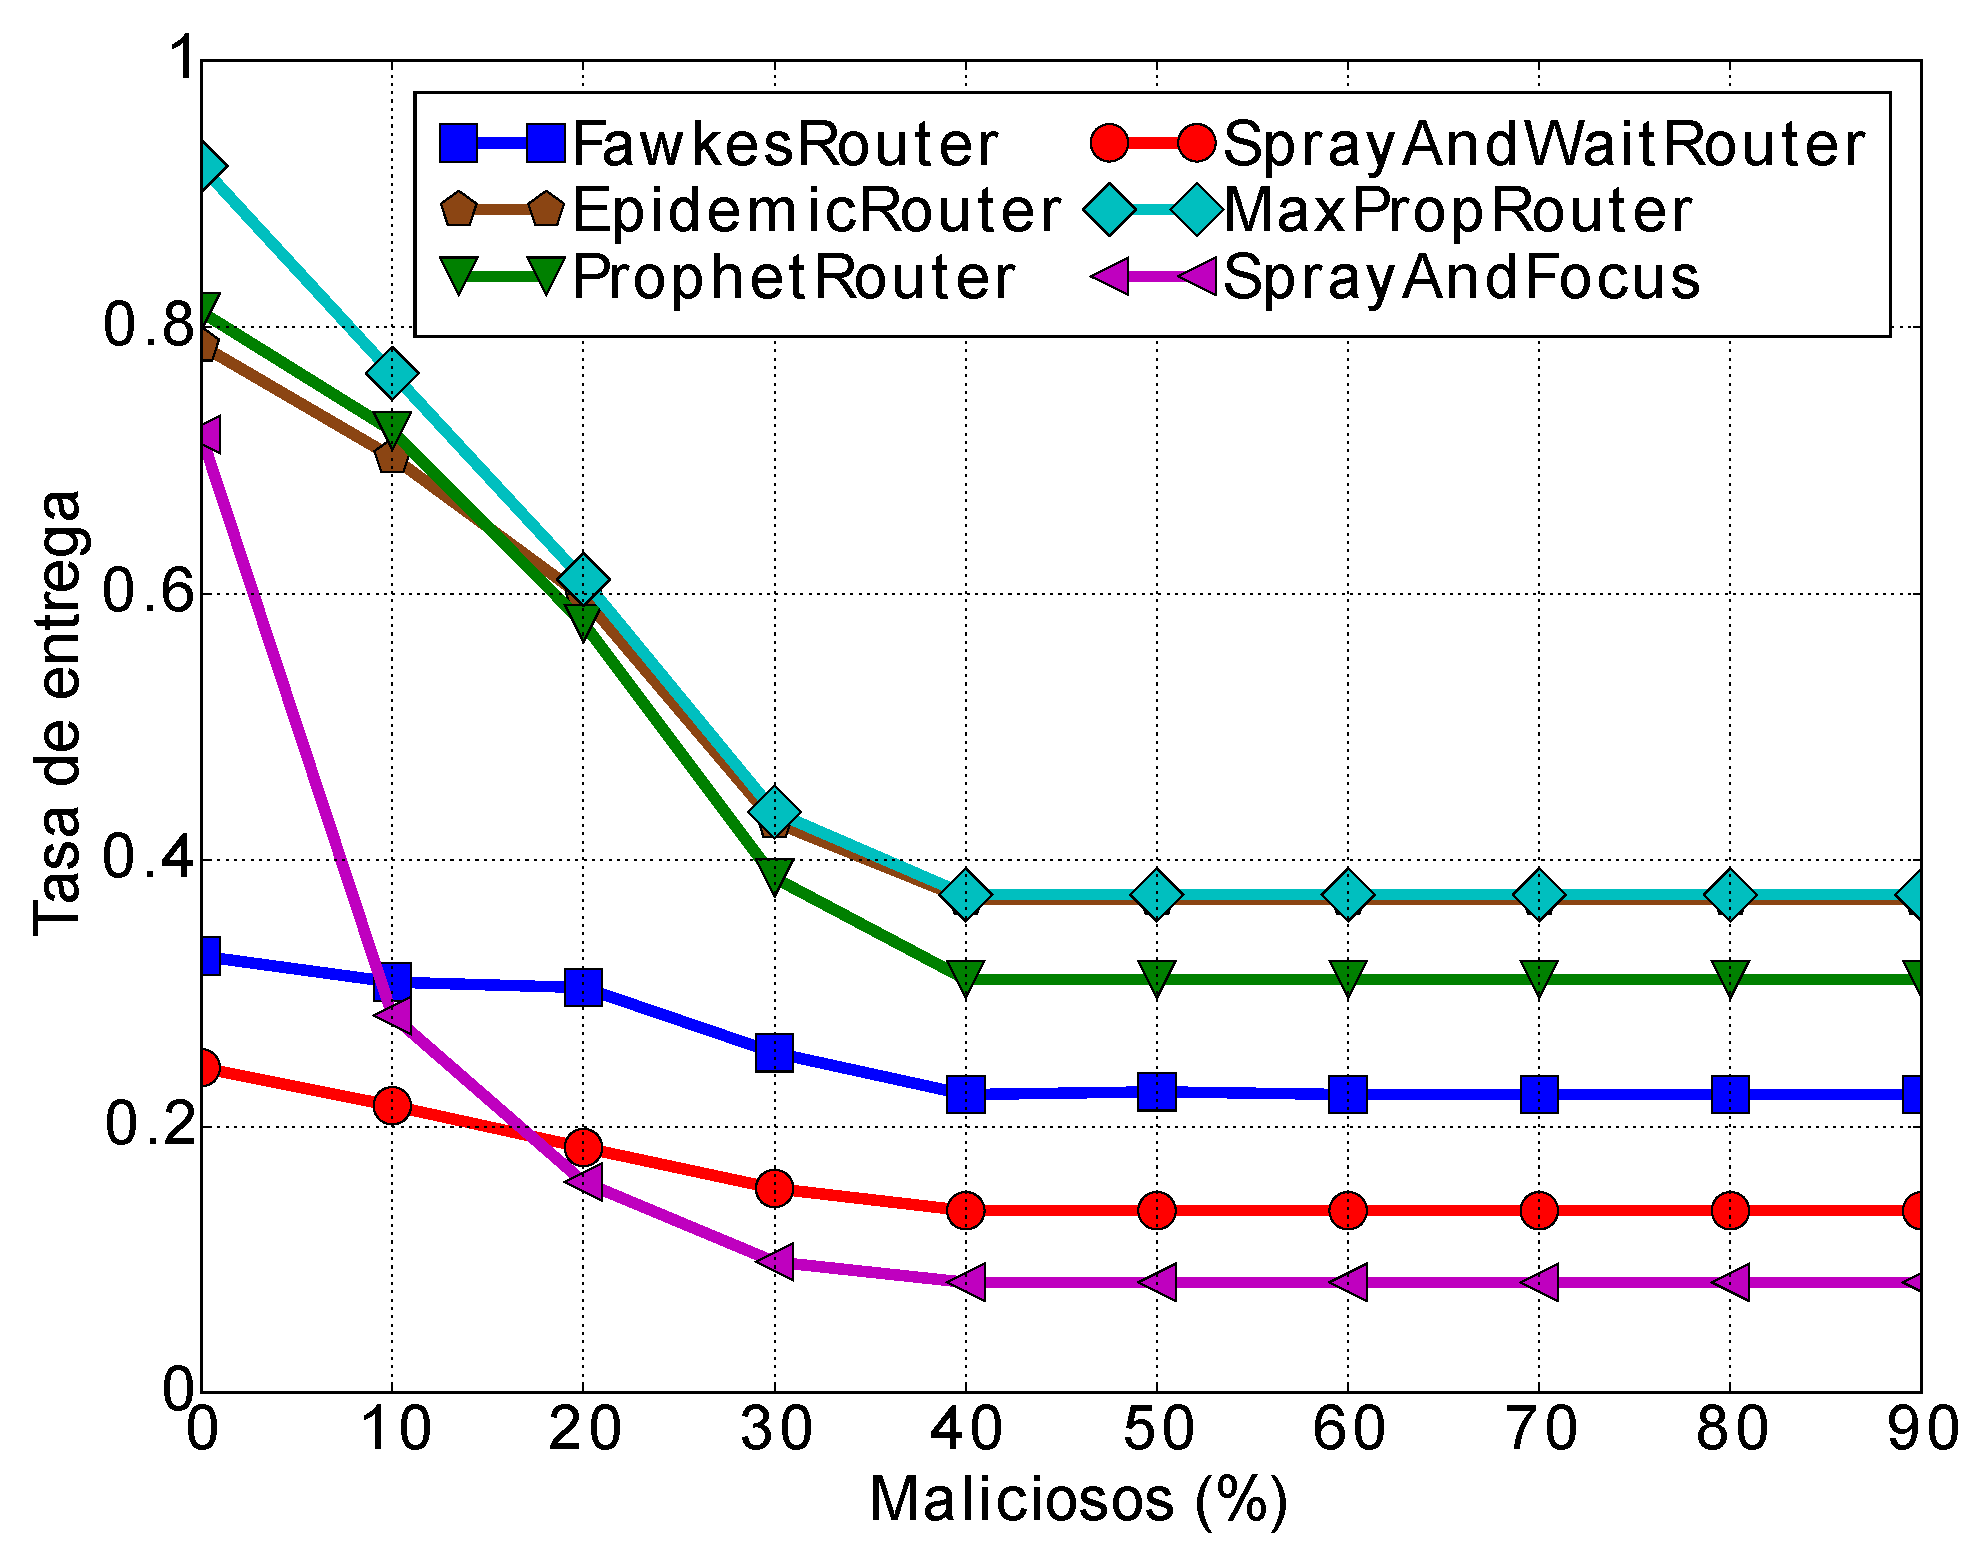
\includegraphics[width=0.6\textwidth]{imagenes/seguridad/graficos/delivery_pdm_todos.eps}}{fig:delivery-protocolos-pdm}
{Elaboración propia, (2015)}

\figuraFuente{\textit{Overhead} en PDM para distintos protocolos.}
{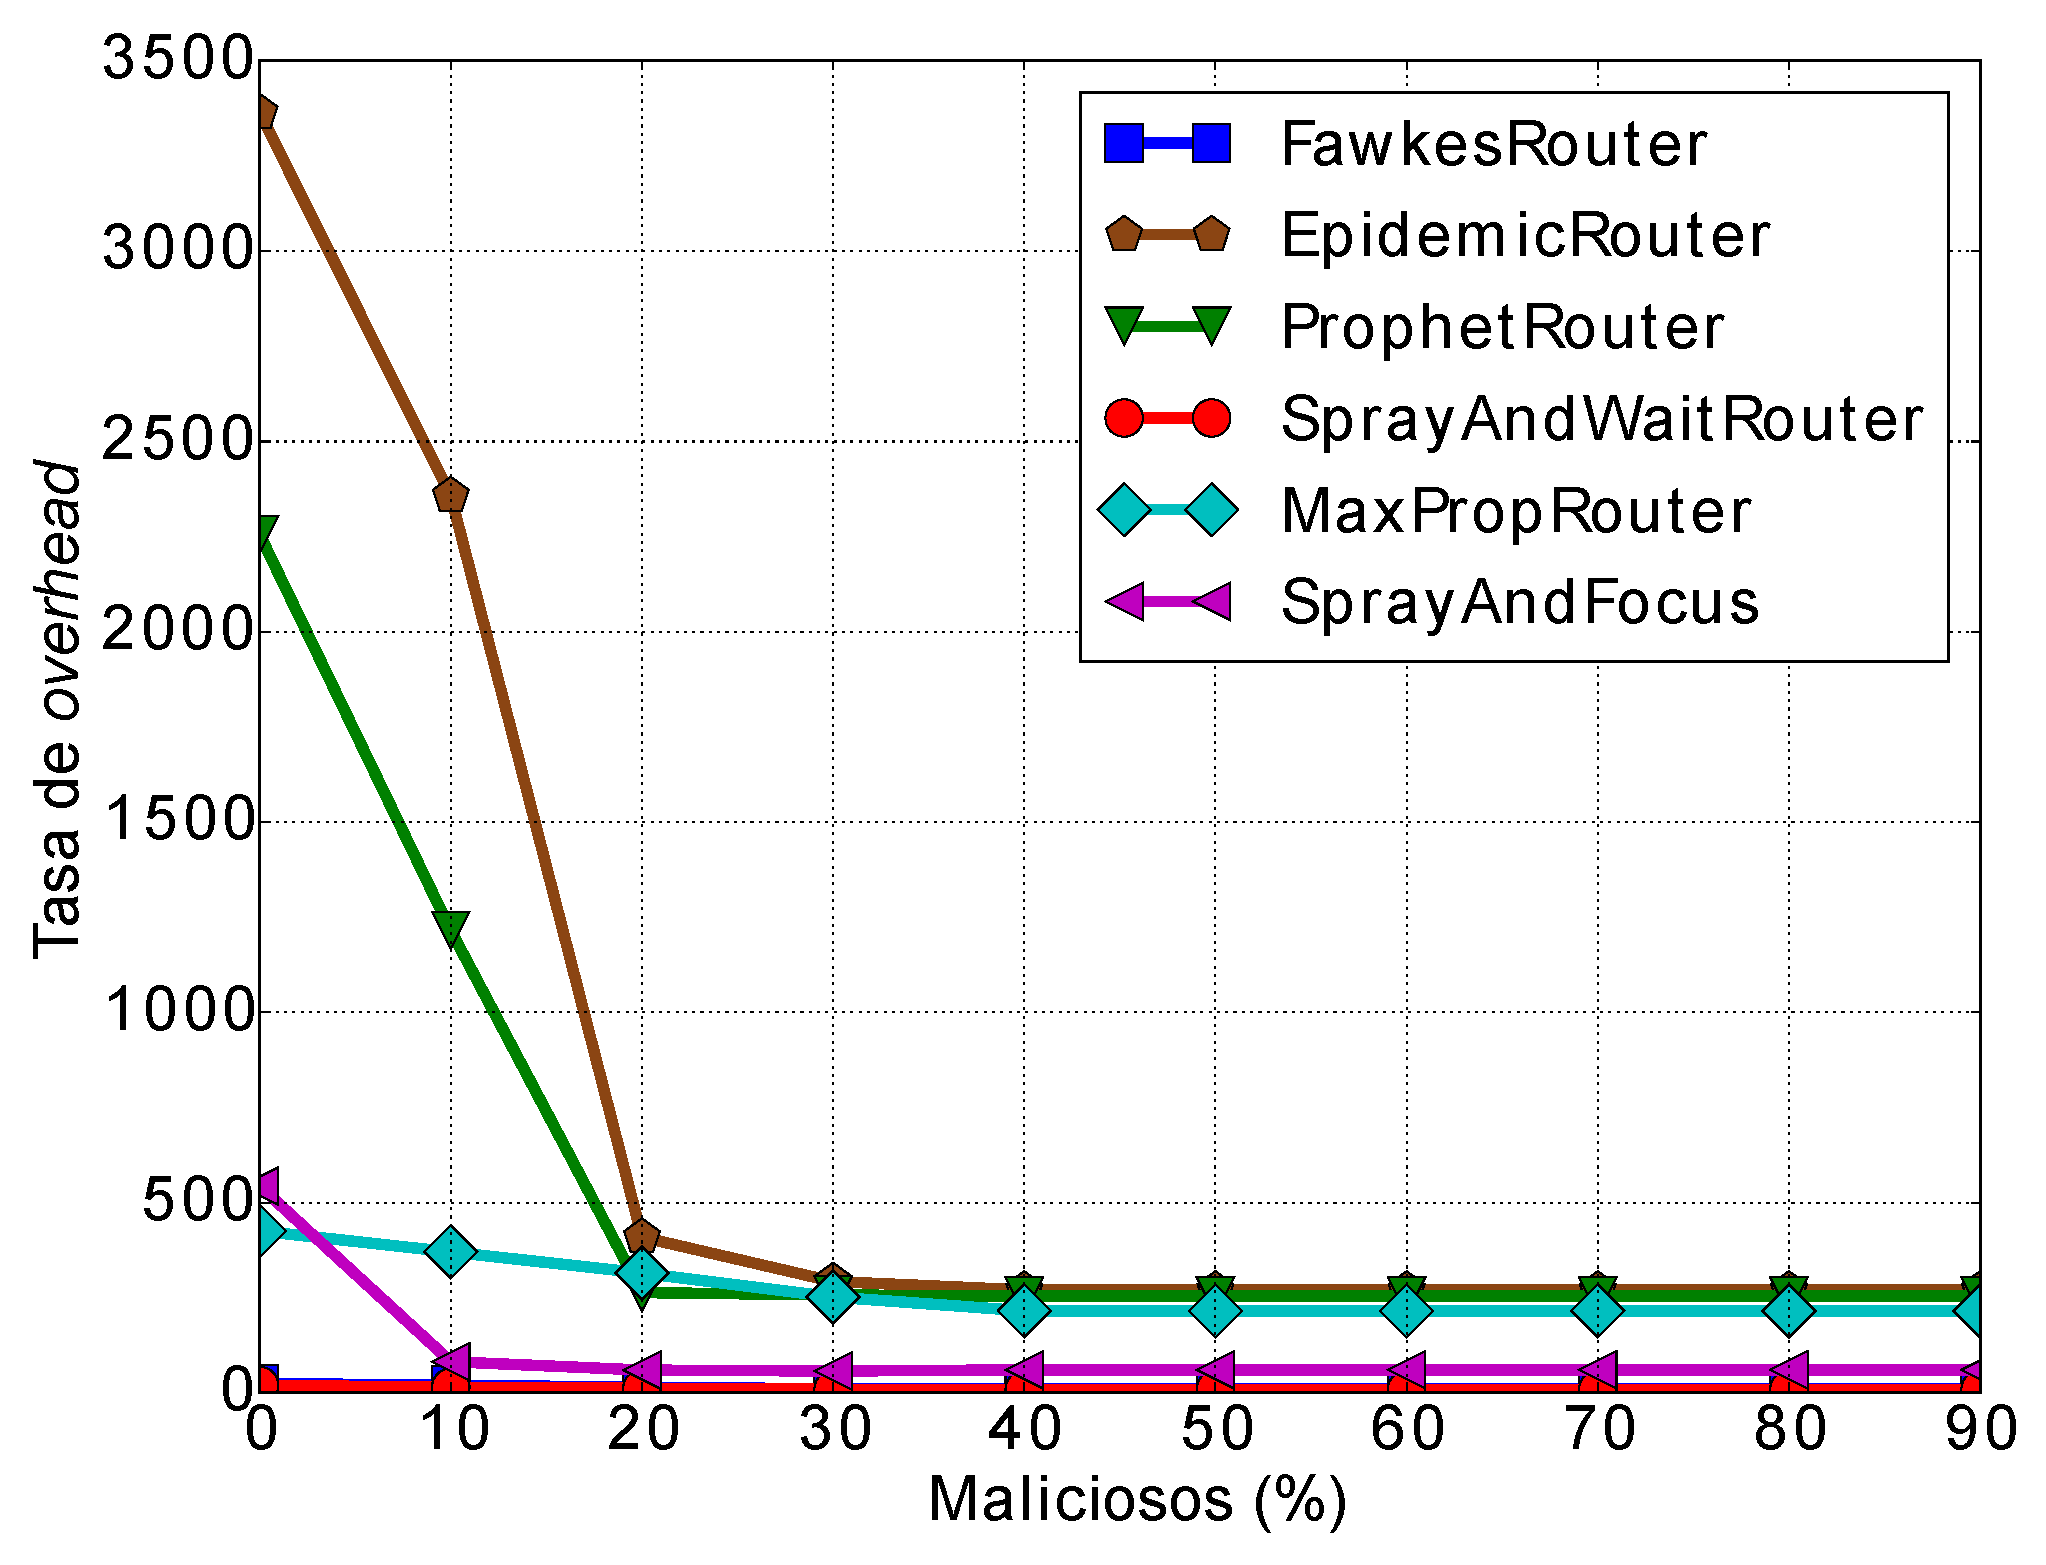
\includegraphics[width=0.6\textwidth]{imagenes/seguridad/graficos/overhead_pdm_todos.eps}}{fig:overhead-protocolos-pdm}
{Elaboración propia, (2015)}

\figuraFuente{Cantidad de mensajes atraídos en PDM para distintos protocolos.}
{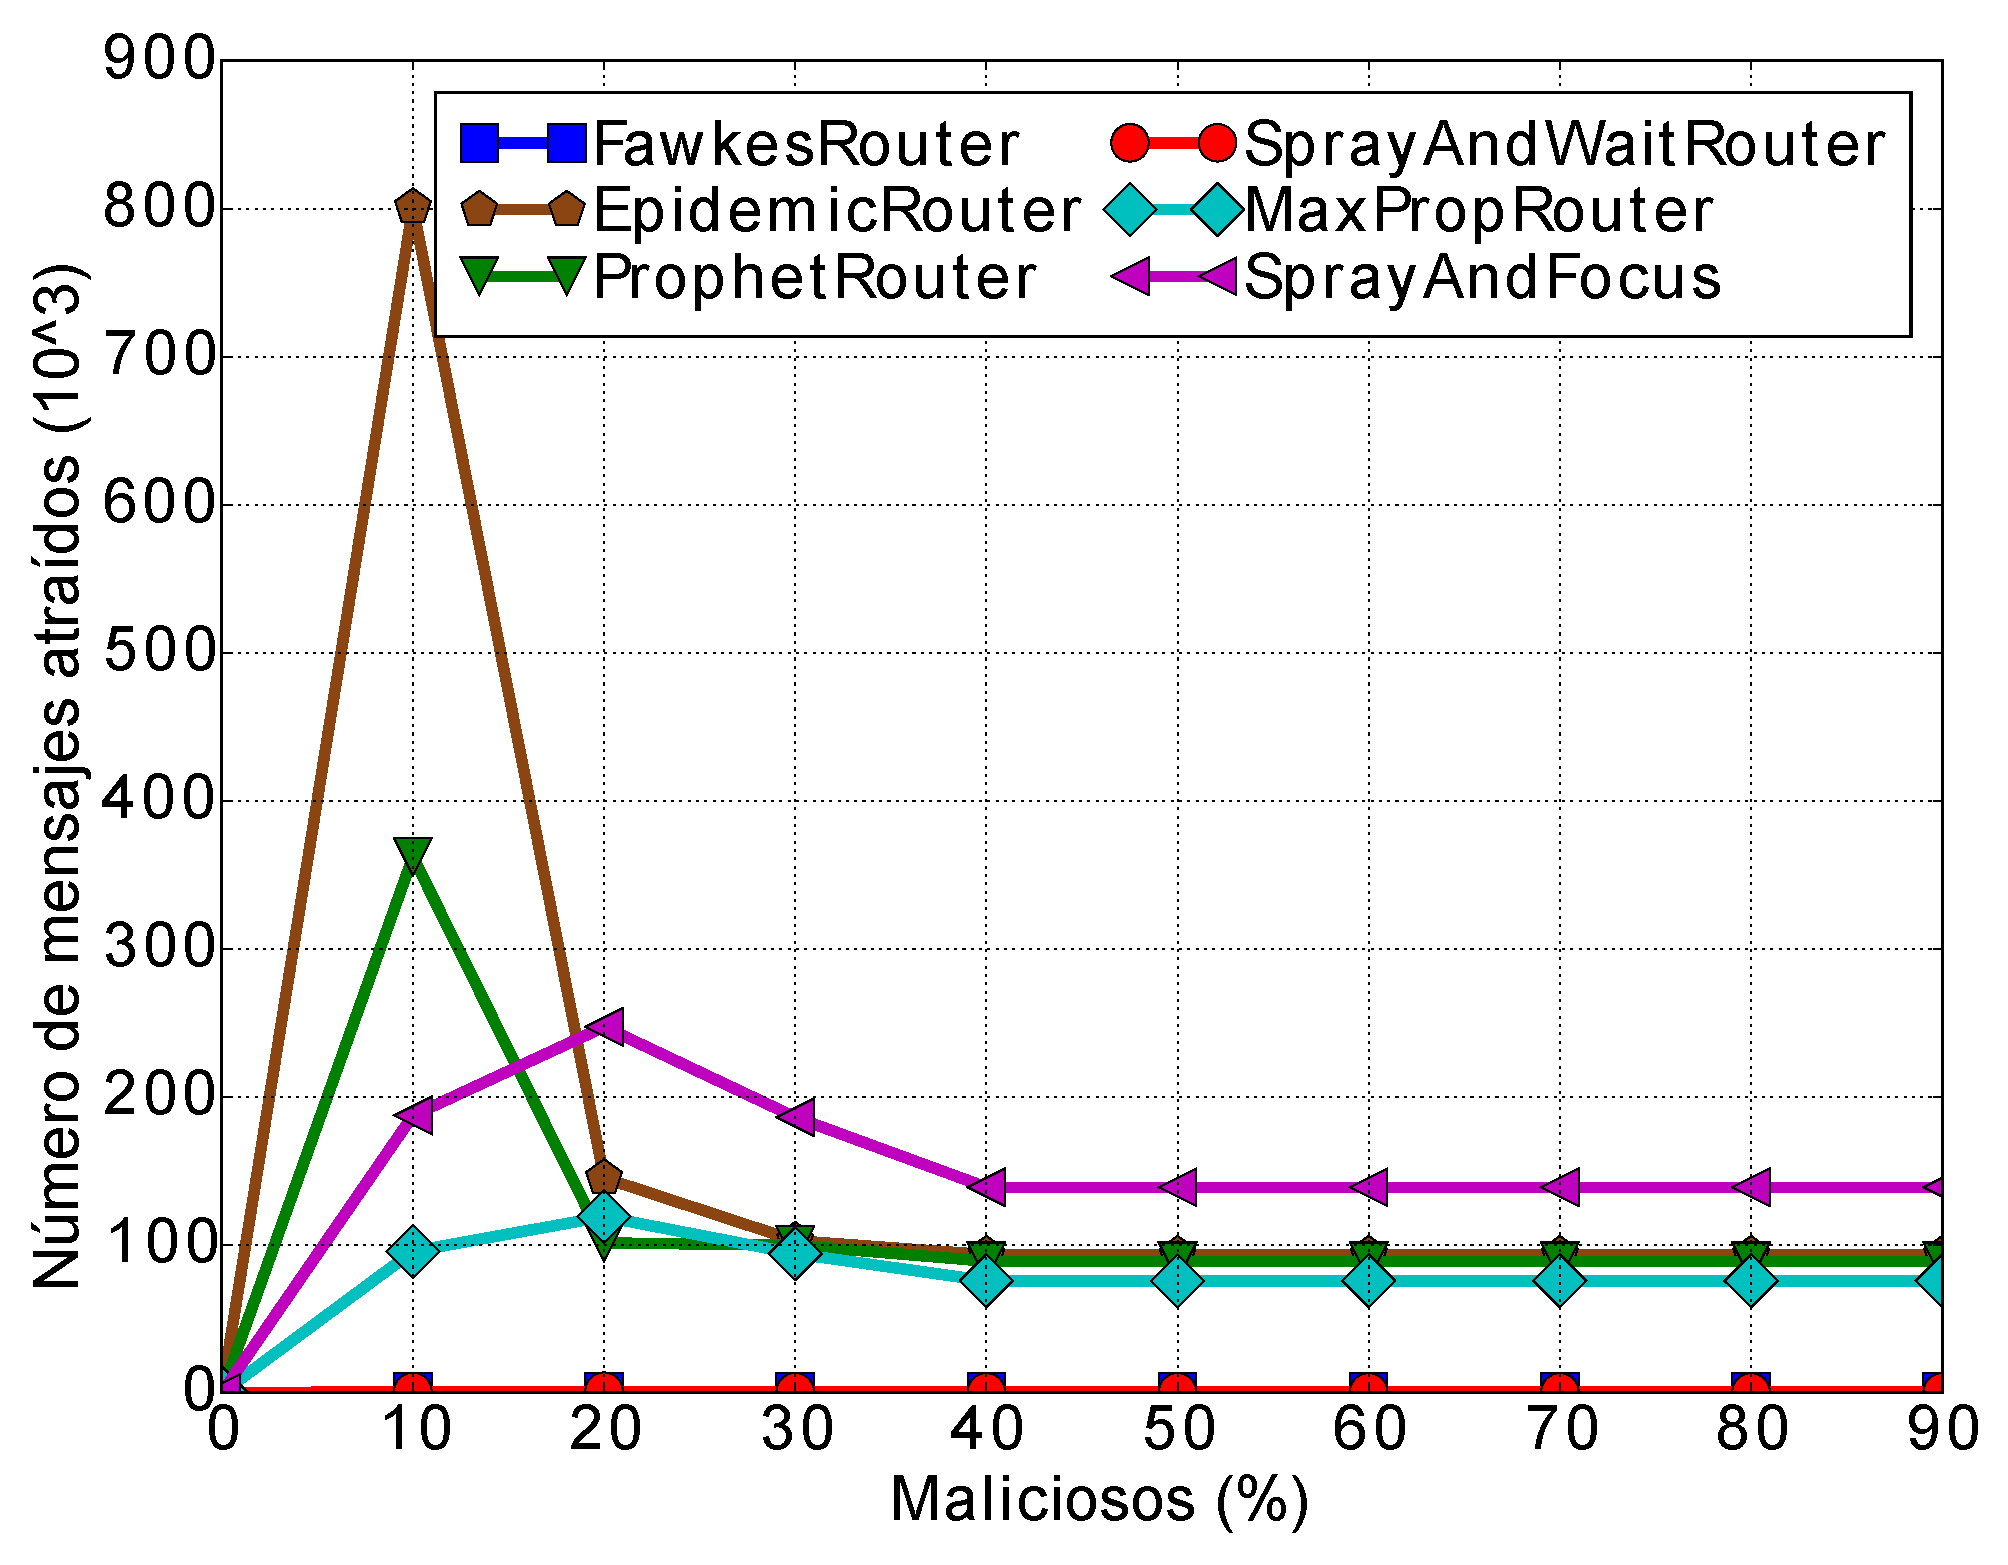
\includegraphics[width=0.6\textwidth]{imagenes/seguridad/graficos/atraidos_pdm_todos.eps}}{fig:atraidos-protocolos-pdm}
{Elaboración propia, (2015)}


%%%%%%%%%%%%%%%%%%%%%%%%%%%%%%%%%%%%%%%%%%%%%%%%%%%%%%%%%%%%%%%%%%%%%%%%%%%%%%%%

Uno de los problemas que surgen de la solución propuesta es el tamaño de las
\textit{hash chains}, las cuales si se dejan crecer sin un límite pueden
provocar el consumo de los recursos de almacenamientos en un dispositivo móvil.
Para prevenir esto, es posible eliminar secciones viejas de la cadena para
liberar espacio, pero entonces aparece el problema de cuanta es la información
mínima que se debe mantener guardada. En la \ref{fig:chains-atraidos} se muestra
como la información disponible afecta el desempeño de \textit{FawkesRouter}.
Cuando se mantienen mensajes con \textit{timestamp} de $1$ o menos horas hay
$1.8*10^3$ mensajes atraídos por los nodos, valor que baja a medida que hay más
información disponible para la toma de decisiones. Esto quiere decir que para
que \textit{FawkesRouter} sea efectivo en la prevención de transmitir menajes a
nodos maliciosos se debe tener al menos $2$ horas de mensajes, tener mensajes
más viejos no mejora de manera significativa el protocolo.

%%%%%%%%%%%%%%%%%%%%%%%%%%%%%%%%%%%%%%%%%%%%%%%%%%%%%%%%%%%%%%%%%%%%%%%%%%%%%%%%


\figuraFuente{Desempeño de las \textit{hashs chains} en el tiempo.}
{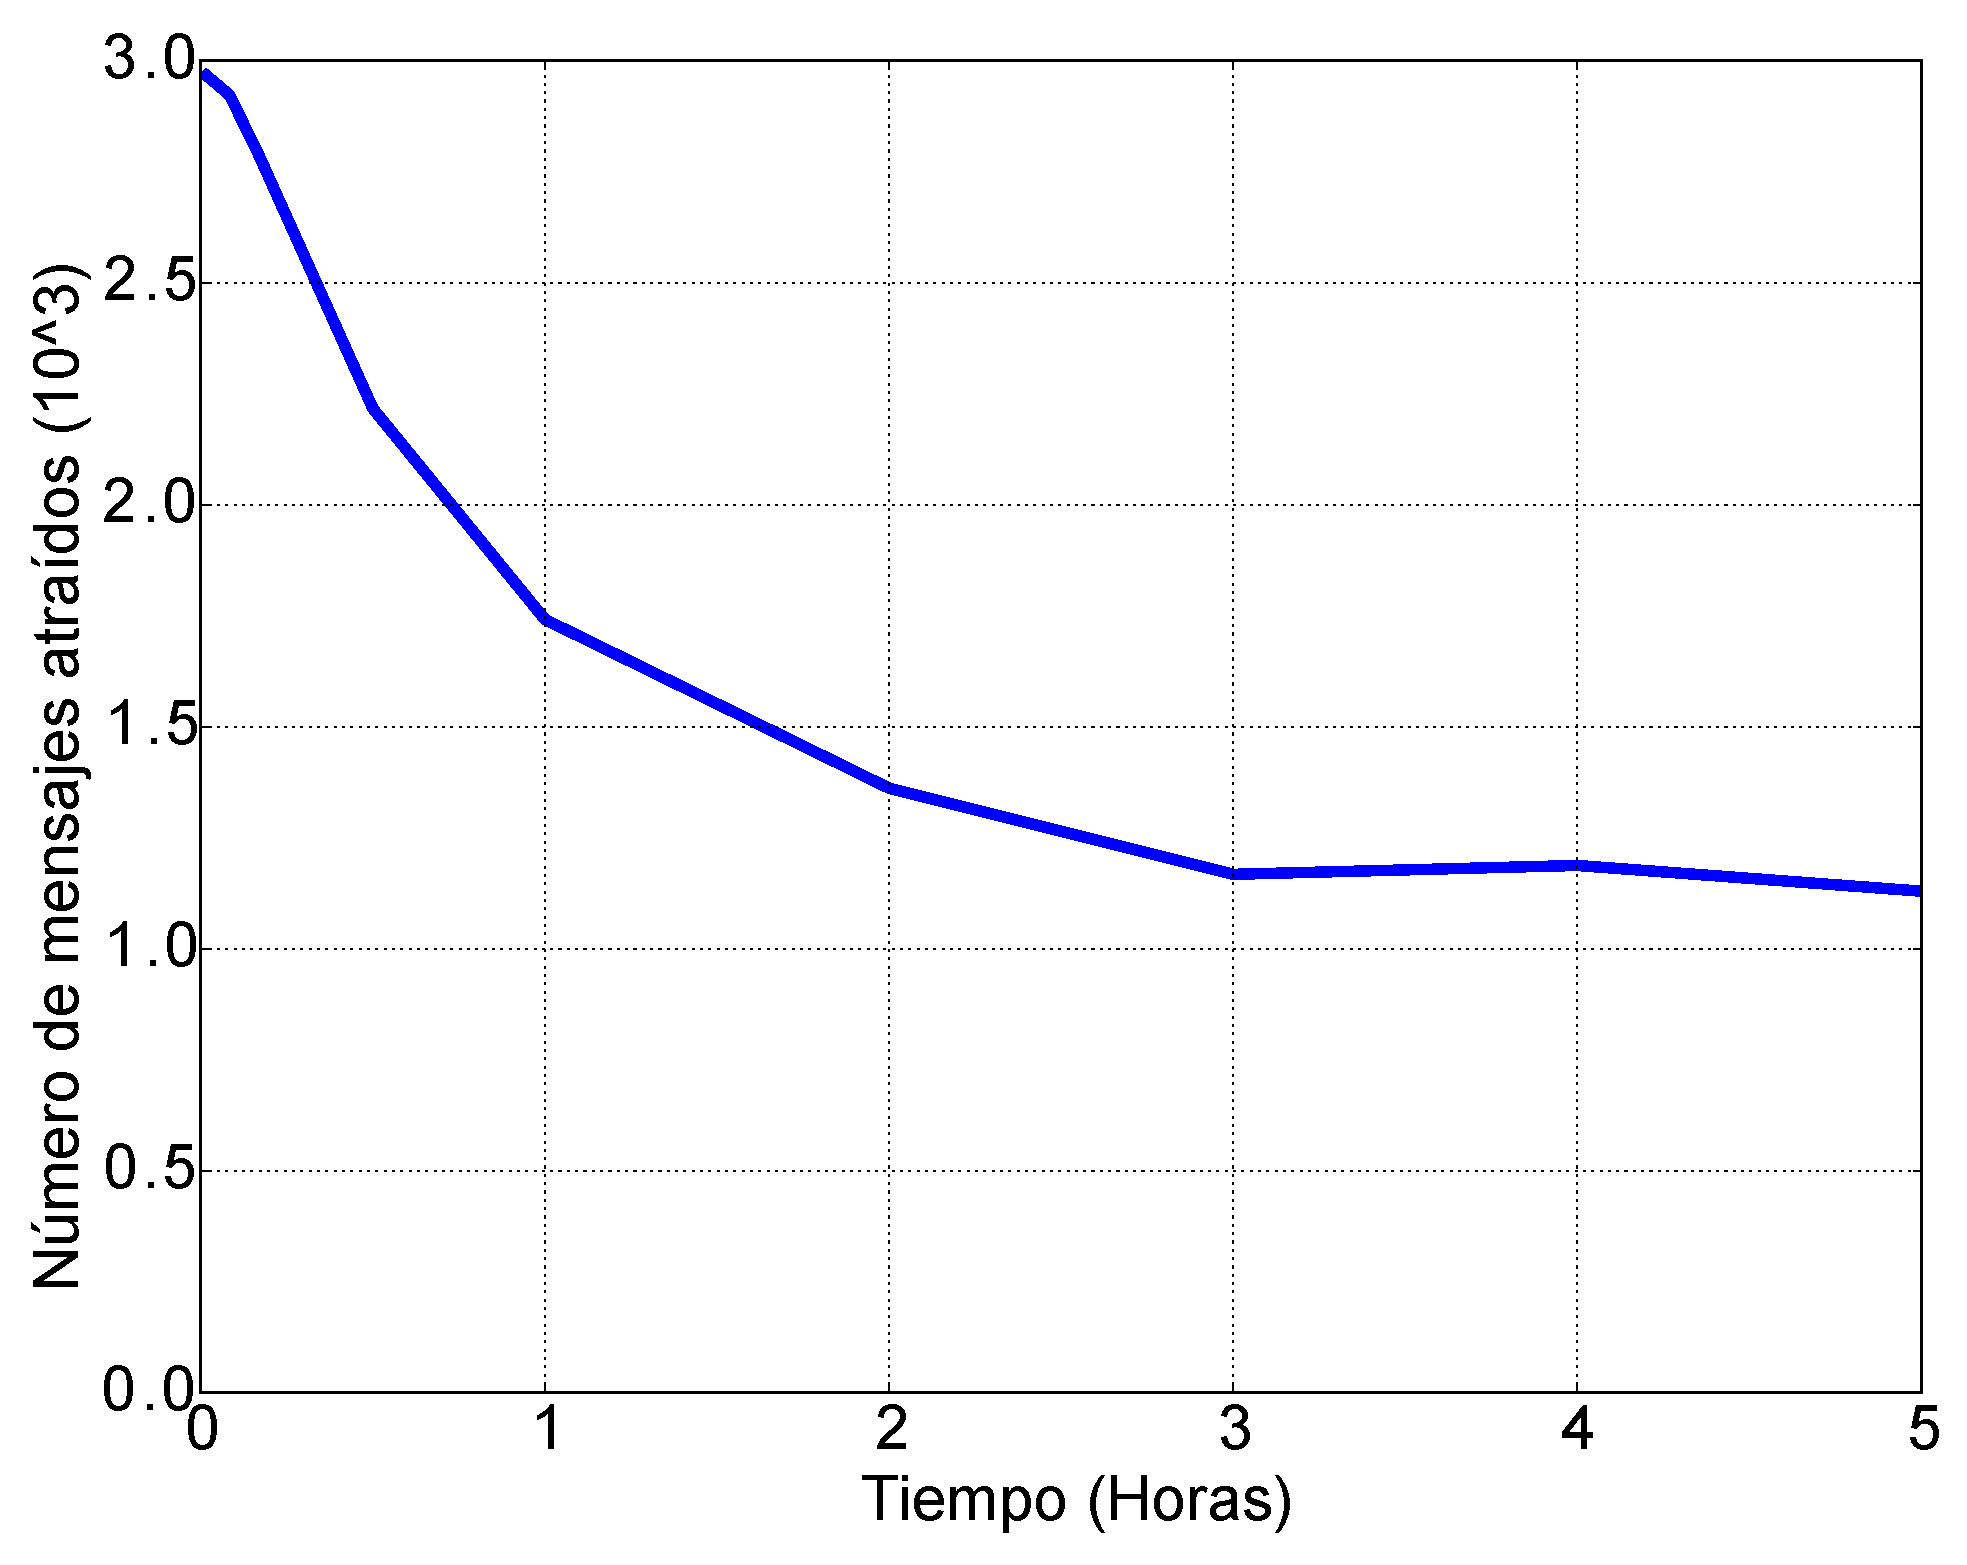
\includegraphics[width=0.6\textwidth]{imagenes/seguridad/graficos/cadenas_atraidos.eps}}{fig:chains-atraidos}
{Elaboración propia, (2015)}




\seccion{Conclusiones}

El protocolos \textit{Guy Fawkes} entrega una forma de autenticar los
\textit{tickets} de interacción sin la necesidad de estar constantemente
comunicado con una PKI, por lo que su uso en \textit{FawkesRouter} ayuda a
evitar la falsificación de encuentros y transmisiones de mensajes, previniendo
los ataques de agujero negro en DTN.

Los resultados muestran que \textit{FawkesRouter} puede reducir el número de
mensajes que son atraídos por nodos atacantes manteniendo una buena tasa de
entrega y bajo \overhead.

Se evaluó el protocolo en dos tipos de escenarios, uno de desastre y otro de una
semana normal en una ciudad, mostrando que el protocolo puede ser aplicado en
otras áreas y no se encuentra restringido solo para escenarios de desastres.
